
\chapter[$\boldsymbol{Wb\overline{b}}$ Cross Section Measurement]{${\expandafter\MakeUppercase W}b\overline{b}$ Cross Section Measurement}\label{sec:wbbxc}

The first of the two processes examined 
 in this thesis is the SM production
 of \ppwbblnbb at \s 8 \TeV, described
 in Section~\ref{sec:wbbproduction}.
Throughout this section, $\ell$ or lepton denotes
 an electron or a muon.

\section{Event Selection}

Two decay channels of the \w boson are considered,
 $\w\rightarrow \mu\nu_\mu$ and $\w\rightarrow e\nu_e$,
 and events are selected using
 single-muon (single-electron) triggers with a
 loosely isolated muon (electron)
 with transverse momentum $\pt>24~(27)$ \GeV
 and pseudo-rapidity $\abs{\eta}<2.1~(2.5)$.
Individual particles emerging from each
 collision are reconstructed with the
 particle-flow (PF) technique described
 in Section \ref{sec:reconstruction}.

Both the muon and electron candidates are required to have 
 $\pt > 30$ \GeV, $\abs{\eta}<2.1$ and
 to originate from the PV of the event,
 as defined in Section \ref{sec:vertexreco}.
These leptons must also pass
 tight ID and isolation requirements,
 with $I < 0.12~(0.10)$ for selected muons
 (electrons) as defined in Equation \ref{eq:iso}.
Additionally, to reject some of the background events
 contributed by processes such as \ppttbar
 and \ppzj, events with more than one 
 lepton {$\pt > 10$} GeV and {$|\eta| < 2.4$}
 are rejected.
Jets are constructed from PF candidates using the
 anti-$k_t$ clustering algorithm \cite{Cacciari:2008gp}
 with a distance parameter of 0.5,
 and jets are $b$-tagged using the multivariate
 discriminator at an operating point
 with a efficiency of 40\% and a misidentification probability of
 0.1\% for light jets and 1\% for charm jets
 described in Section \ref{sec:jetsvreco}.
Exactly two $b$-tagged jets with
 {$\pt > 25$} GeV and {$|\eta| < 2.4$} are required
 to be present in selected events, to 
 remove contamination in the signal region from 
 charm and light flavor jets.
To reduce the contribution from \ppttbar events,
 events  with
 a third jet with {$\pt > 25$} GeV and {$|\eta| < 4.7$}
 are rejected.
The effects of the various cuts with regard to the 
 total number of events passing selections on the data 
 is illustrated in Table \ref{tab:wbbcutflow}.

\begin{table}
\caption[\wbb Cutflow]
{
Listed below are the raw number of events in data 
 passing the selection listed in the first column
 as well as all selections in higher rows.
The second column is for the \wmn decay channel, 
 and the third column is for \wen.
}
\begin{center}
\begin{tabular}{r|l|l}
{}         & \multicolumn{2}{c}{Events passing selection} \\
Selection  & \wmn & \wen \\
\hline\hline
 $\pt^{\ell_1} > 30$ \GeV and $\abs{\eta^{\ell_1}}<2.1$           & X  & X \\
 $\pt^{\ell_2} \ngtr 10$ \GeV or $\abs{\eta^{\ell_2}}\nless 2.1$  & X  & X \\
 {$\pt^{j_1,j_2} > 25$} GeV and {$|\eta^{j_1,j_2}| < 2.4$}        & X & X \\
 {$\pt^{j_3} \ngtr 25$} GeV or {$|\eta^{j_3}| \nless 4.7$}        & X & X \\
 $b$-tag $j_1,j_2$                                                & X & X
\end{tabular}
\end{center}
\label{tab:wbbcutflow}
\end{table}


\section{Simulated samples}

After all selection requirements
 detailed in Section \ref{sec:wbb_analysisstrategy} are applied,
 the contributing processes to the overall yield are the
 associated production of a massive vector boson and jets (\vjets),
 as well as diboson ($WW$, $WZ$, $ZZ$), $\ttbar$,
 single top quark, \gjets, and QCD multijet production.
The corresponding contributions are estimated from simulation,
 except for the QCD background, which
 is estimated from data as described in Section \ref{sec:qcd}.


Simulated samples of \vjets, \gjets
 and  \ttjets are generated at tree-level with
 \textsc{\MADGRAPH~5.1} \cite {Alwall:2011uj,ref:MadEvent} % \cite{ref:MadEvent,Alwall:2007st,Alwall:2011uj}
 using the CTEQ6L \cite {ref:CTEQ66} Parton Distribution Function (PDF) set.
These samples are interfaced with
 \textsc{\PYTHIA~6.4} \cite {Sjostrand:2006za} using the Z2* tune
 for hadronization.
The most recent \textsc{\PYTHIA} Z2* tune is derived from the Z1 tune \cite {Field:2010bc},
 which uses the CTEQ5L parton distribution set, whereas Z2* adopts CTEQ6L \cite {ref:CTEQ66}.
The $k_t$-MLM \cite {Alwall:2007fs,Alwall:2008qv} matching scheme is used.
For the signal distributions, the \wbb component of
 an inclusive \wjets sample is used,
 with the shapes of the distributions taken
 from a dedicated high-statistics generated sample of exclusive \wbb.
The shape of the \wbb signal distribution is obtained by separating
 the \wjets simulated sample into three subsamples labeled as \wbb, \wcc, and \wudscg.
These three categories are described below.
The separation is done at the particle list level.
If an event contains a $b$ jet, from the matrix element or parton shower,
 it falls into the \wbb category.
A $b$ quark at generator level requires
 the presence of a $b$ hadron within a cone of
 radius $R=0.4$ with respect to the jet axis.
The jets are constructed using generator-level information using
 all stable particles in the event excluding neutrinos.
Jets with a distance smaller than $R = 0.5$ with respect to a
 lepton are removed from the event.
%Exactly two $b$ jets with $\pt>25\GeV$ and $|\eta|<2.4$
% are required in the signal region.
If an event contains no $b$ jets, but
 an even, non-zero, number of charm jets,
 again from the matrix element or
 parton shower, it falls into the \wcc category.
The remaining events fall into the \wudscg category.
% hen level definitions
The energy of the selected leptons at the generator level is corrected
 for final-state radiation by summing up
 the four-momenta of
 all the photons generated within a cone of radius $R = 0.1$
 around the lepton.
Generated leptons which do not originate in simulation
 from the primary interaction vertex are not considered for selection.

Single top quark event samples are generated at next-to-leading order (NLO) with
 \textsc{\POWHEG~2.0} \cite {Nason:2004rx,Frixione:2007vw,ref:POWHEG_T_SandTchannel,ref:POWHEG_T_tWchannel}
 %\POWHEG 2.0 \cite{Nason:2004rx,Frixione:2007vw,Alioli:2008gx,ref:POWHEG_T_SandTchannel,ref:POWHEG_T_tWchannel}
 using the CTEQ6M PDF set.
Hadronization is performed using
 \textsc{\PYTHIA~6.4} with the Z2* tune.
Diboson samples are generated and hadronized
 with \textsc{\PYTHIA~6.4} at leading order (LO)
 using the CTEQ6L PDF set and the Z2* tune.

The cross sections for the \vjets and \gjets processes
 are normalized using the predictions
 for inclusive W, Z and photon production from
 \textsc{fewz~3.1} \cite {Gavin:2012sy,ref:FEWZ3.1}
 evaluated at next-to-next-to-leading order (NNLO).
Single top quark and diboson production cross sections are
 normalized to the NLO
 cross section predictions from $\MCFM~7.0$ \cite {Campbell:2010ff, Badger:2010mg}
 using the MSTW08 NLO PDF set \cite{Martin:2009iq}.
The $\ttbar$ cross section used is $241.5\pm8.5$ pb and
 was determined from data collected by the ATLAS and CMS
 experiments \cite{CMS:2014gta,Aad:2014kva,Chatrchyan:2013faa}
 at the LHC at $\sqrt{s}=8\TeV$.


Events induced by additional simultaneous pp interactions
 are simulated using events generated with \textsc{\PYTHIA~6}.
During the 2012 data taking, the average pileup rate was
 21 interactions per bunch crossing and
 the simulated number of pileup interactions
 have been reweighted to match this distribution in the data.


\section{Background Estimation}

\subsection{QCD}
\label{sec:qcd}
The QCD multijet sample is derived using a data-driven method. 
The shapes of the distributions for QCD multijet events are taken as the difference between
 the data sample and the sum of the other simulated backgrounds in a region of phase
 space enriched in multijets as illustrad in Figure \ref{fig:qcdshape}.
This region is found using the same selection requirements as those in the signal region,
 but requiring the muon (electron) to be antiisolated: $I > 0.20 \; (0.15)$.
In the fiducial regions used in this analysis,
 no correlation is observed between $I$ and $\mt$, validating
 the use of an inverted isolation requirement to obtain
 the QCD background shape.
This is not the case for the $\Delta R$ distance between the
 two $b$-tagged jets, $\Delta R(b,\bar{b})$, or the lepton $\pt$.
The shape of the QCD distribution for these variables is therefore
 taken from an $\mt<30$ \GeV sideband and validated against
 QCD multijet simulation.
The normalization of the QCD background
 in these variables is set to the final
 normalization resulting from the fit to the \mt variable
 which was derived using the inverted isolation requirement.
To obtain an initial estimate of the number of QCD multijet
 events passing signal region selections, the
 shape derived in the antiisolated region, is
 put in the signal region and scaled by $ (d_{20}-m_{20})/q_{20} $ where
 $d_{20}$ is the yield in data in the range $0<\mt<20$, $m_{20}$ is the combined
 yield from the simluated samples in this range, and $q_{20}$ is the corresponding
 unnormalized yield of QCD multijet events.
This has the effect of normalizing the QCD sample such that the combination of the QCD 
 and the simulated backgrounds has the same total yield as data in the range $0<\mt<20$.
If $d_{20}<m_{20}$, the QCD contribution is taken to be negligable. % and is scaled by $10^{-6}$.
% this happens for ttbar multi-lepton
The relative uncertainty in the yield of QCD multijet events is
 estimated to be $\pm$50\%, taking into account both the fit result
 and the extrapolation from $0<\mt<20$ to the high-$\mt$ range.
This relative uncertainty also covers shape mismodelings
 of the multijet contribution in the final sample.


\begin{figure}
 \caption[QCD shape for \wbb analysis]
 {The shape for the QCD is found by inverting the lepton
  isolation and subtracting MC from the data.
  Shown above is the data, MC background and 
   extrapolated QCD shape (difference between data
   and MC backbrounds) for both the muon and electron channels
   in the $W+jj$ and $W+b\bar{b}$ phase spaces.
  The requirement of two well-identified $b$ tags
   essentially eliminates all MC backgrounds in
   the $W+b\bar{b}$ region, leaving the QCD shape 
   the same as that of the data.
  }
 \center
\label{fig:qcd_mu}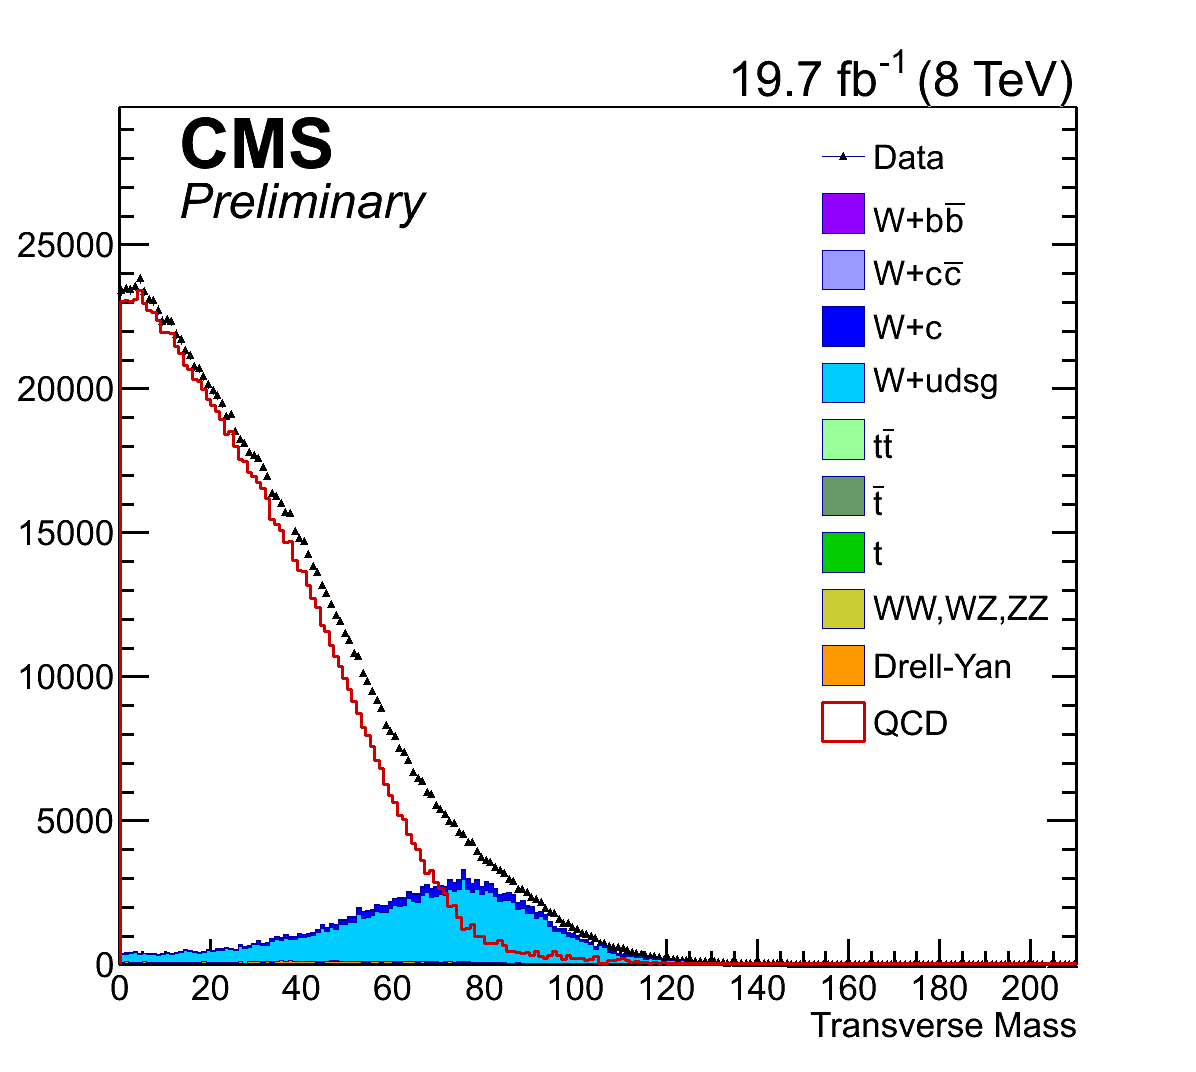
\includegraphics[width=0.4\textwidth]{/Users/rhombus/CMS/Thesis/thesis/pdfs/wbbxc/qcd/QCDShape_wjj_mt_mu.png}
\label{fig:qcd_mu}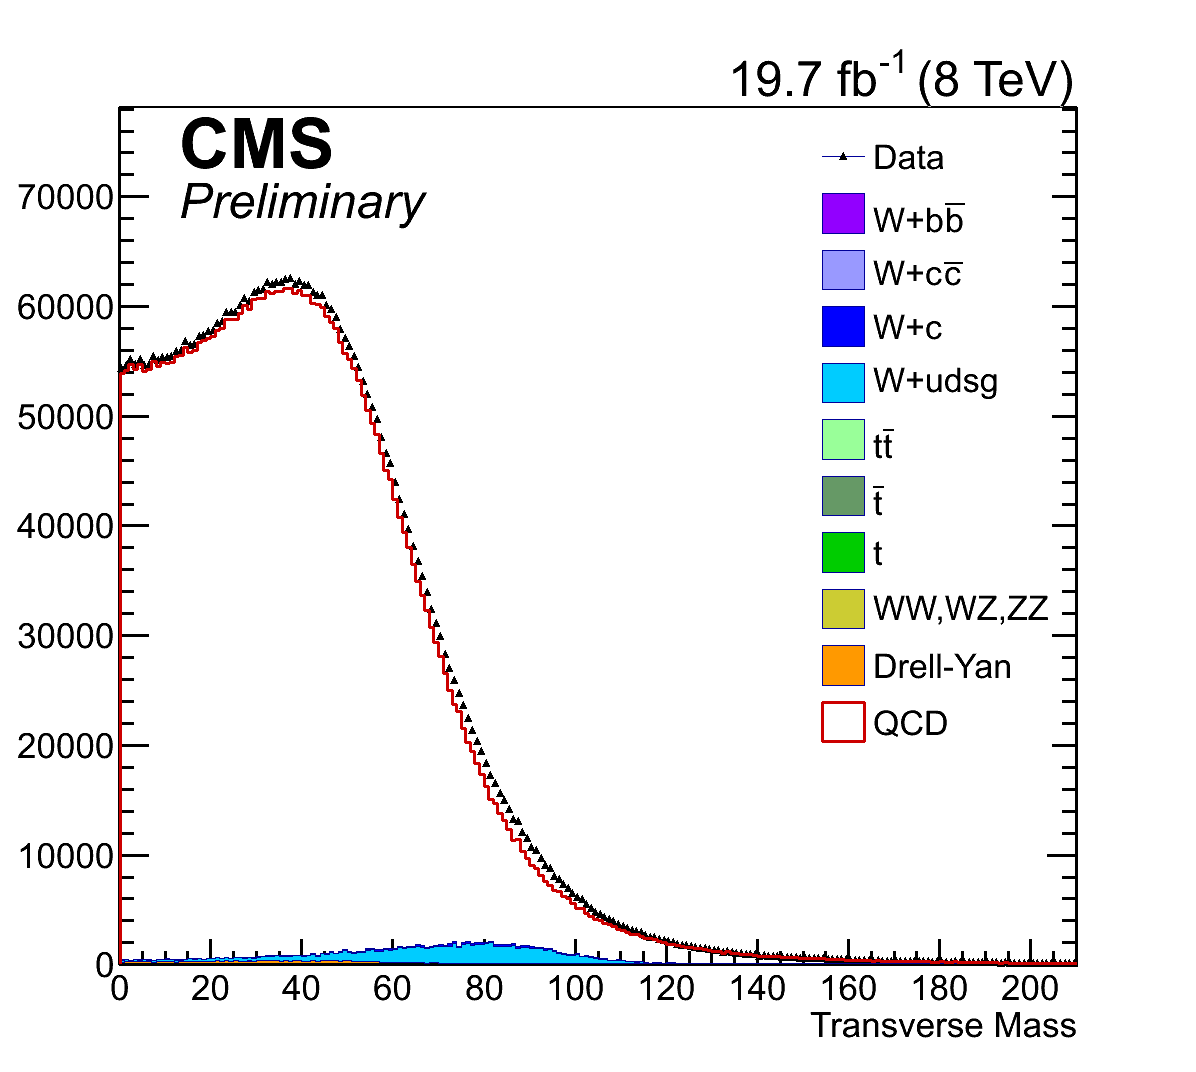
\includegraphics[width=0.4\textwidth]{/Users/rhombus/CMS/Thesis/thesis/pdfs/wbbxc/qcd/QCDShape_wjj_mt_ele.png}
\label{fig:qcd_mu}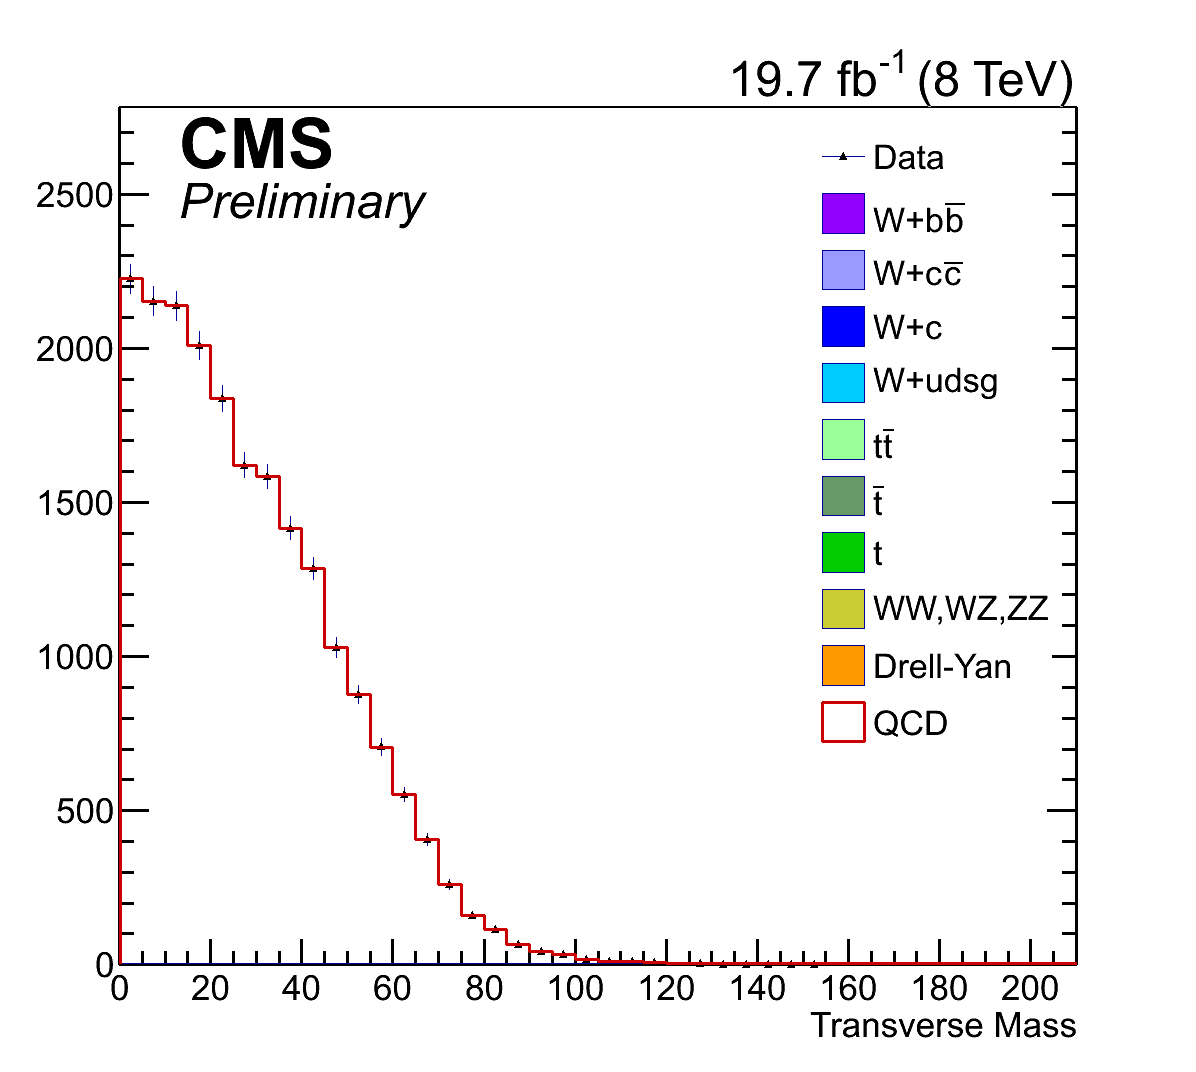
\includegraphics[width=0.4\textwidth]{/Users/rhombus/CMS/Thesis/thesis/pdfs/wbbxc/qcd/QCDShape_wbb_mt_mu_05.png}
\label{fig:qcd_mu}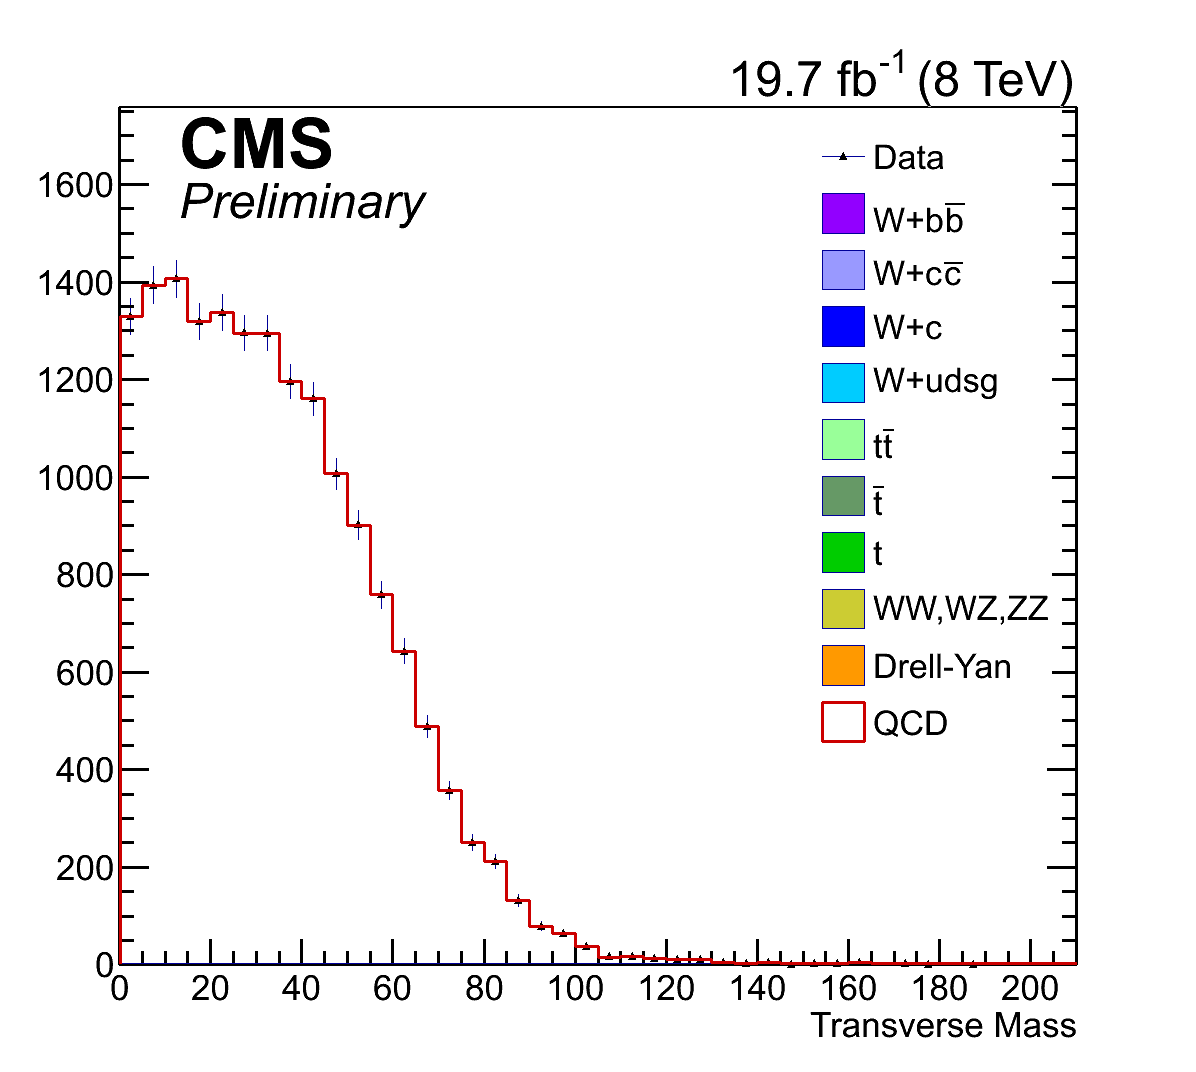
\includegraphics[width=0.4\textwidth]{/Users/rhombus/CMS/Thesis/thesis/pdfs/wbbxc/qcd/QCDShape_wbb_mt_ele_05.png}
 \label{fig:qcdshape}
\end{figure}


\subsection[$W$+jets: light and charm component]
{$\boldsymbol{W}$+jets: light and charm component}

$W$+light jets is the dominant background in the $\wjj$ phase space,
 which is found using idential selections as are used in 
 the signal region with the exception of the $b$ tag requirement.
In the $W+jj$ phase space, no requirements on $b$ tags are made.
This control region therefore serves as a cross check on the 
 reconstructed objects observed in the signal region before
 the added complication of $b$-tagging has been introduced. 
In Figure~\ref{fig:wjj_plots} is shown the \pt 
 of the identified lepton along with the \met and \mt
 in both decay channels.
Agreement between simulation and data is on the order of 10\%.

\begin{figure}
 \caption[\wjj control region for the \wbb measurement]{
  Selecting for a tight ID muon with $\pt>$30 GeV and exactly two central jets passing loose ID,
   we recover the distributions shown above. 
  Shown in the upper left (right)
   is the momentum of the leading lepton in the muon (electron) channel.
  The missing transverse energy is shown in the center,
  and transverse mass is given in the bottom two distributions.
  The shaded band in ratio plots shows statistical uncertainty. 
 } 
\begin{centering}
\begin{tabular}{cc}
 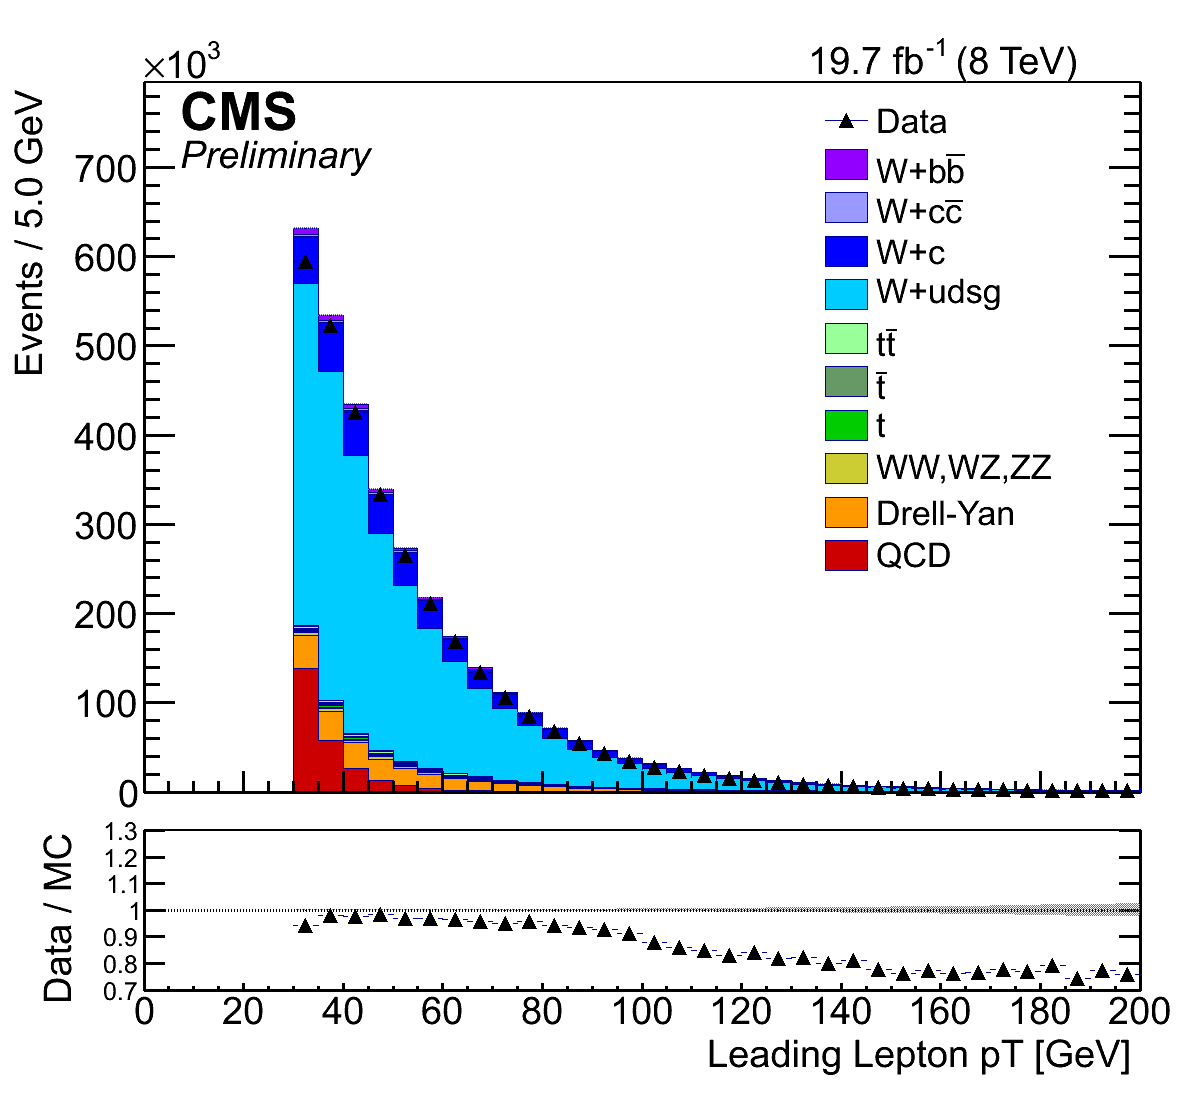
\includegraphics[width=0.4\textwidth]{/Users/rhombus/CMS/Thesis/thesis/pdfs/wbbxc/wjj/Histograms_wjj_goodLep_pt_mu.png} &
 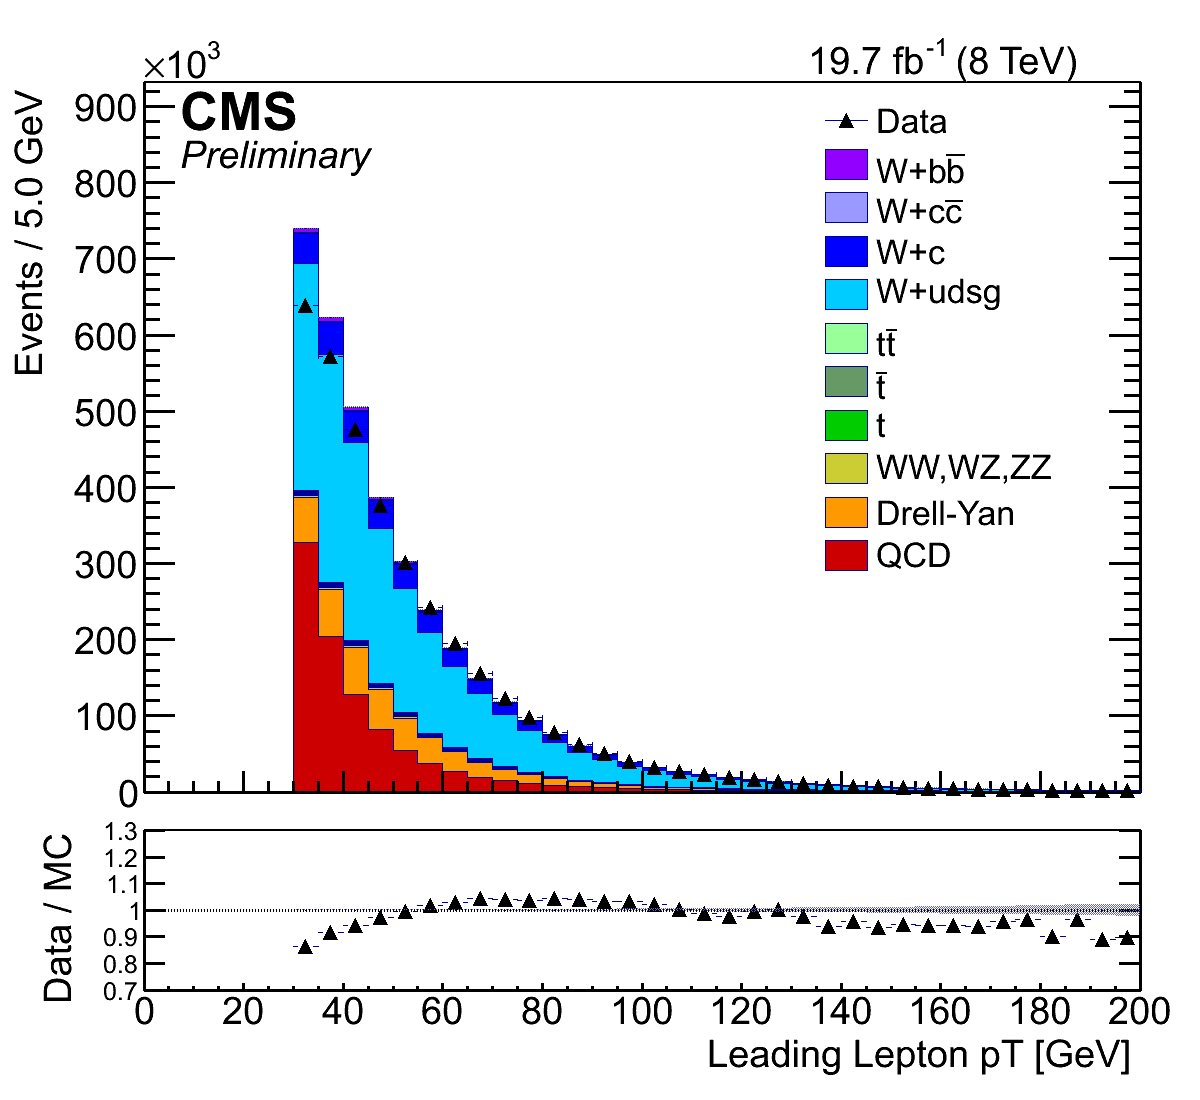
\includegraphics[width=0.4\textwidth]{/Users/rhombus/CMS/Thesis/thesis/pdfs/wbbxc/wjj/Histograms_wjj_goodLep_pt_ele.png} \\
 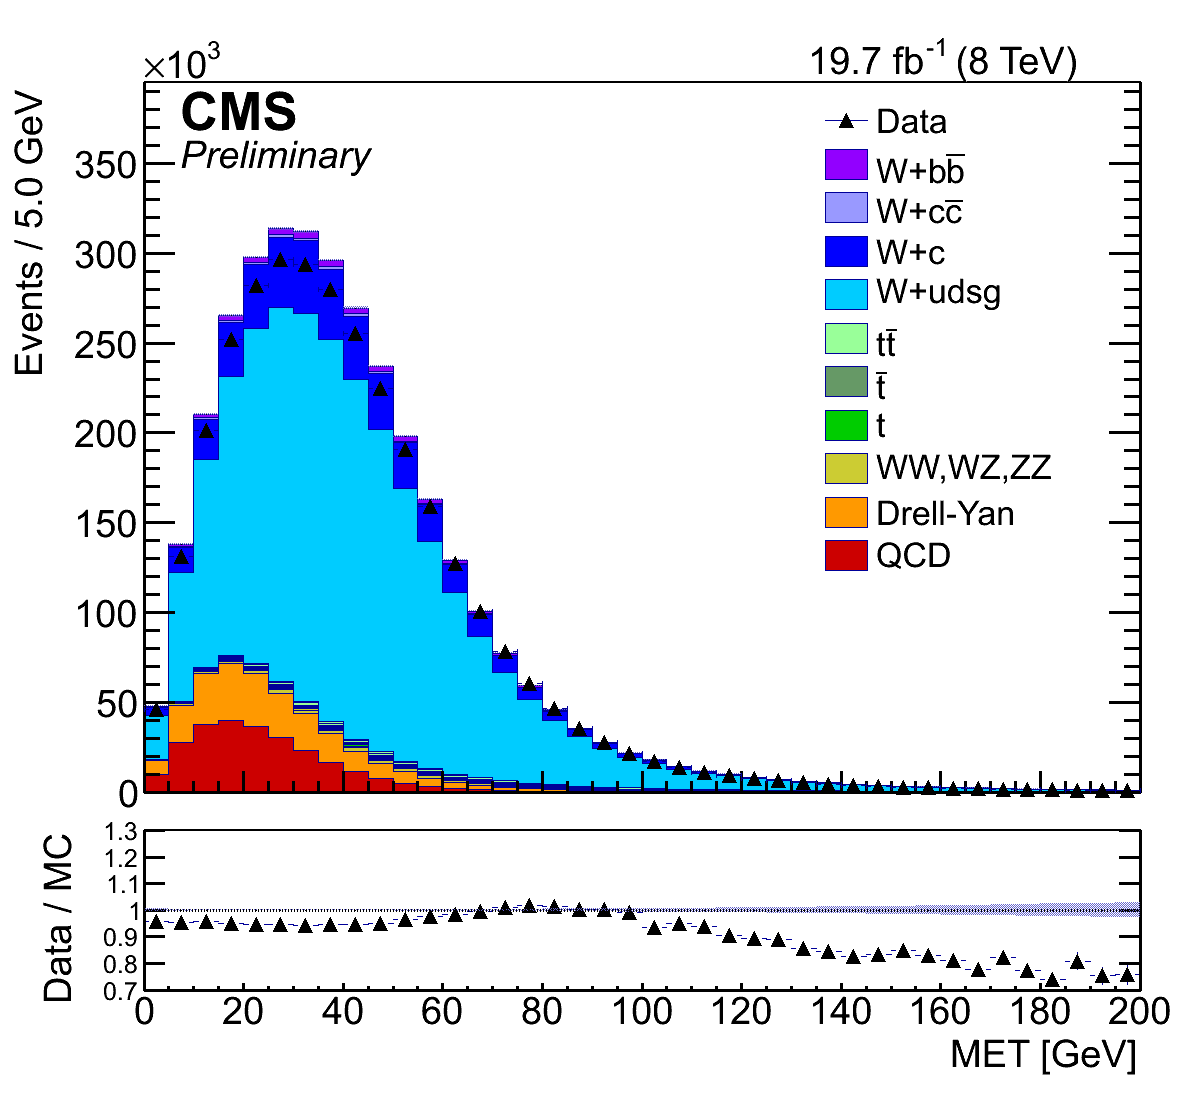
\includegraphics[width=0.4\textwidth]{/Users/rhombus/CMS/Thesis/thesis/pdfs/wbbxc/wjj/Histograms_wjj_met_mu.png} & 
 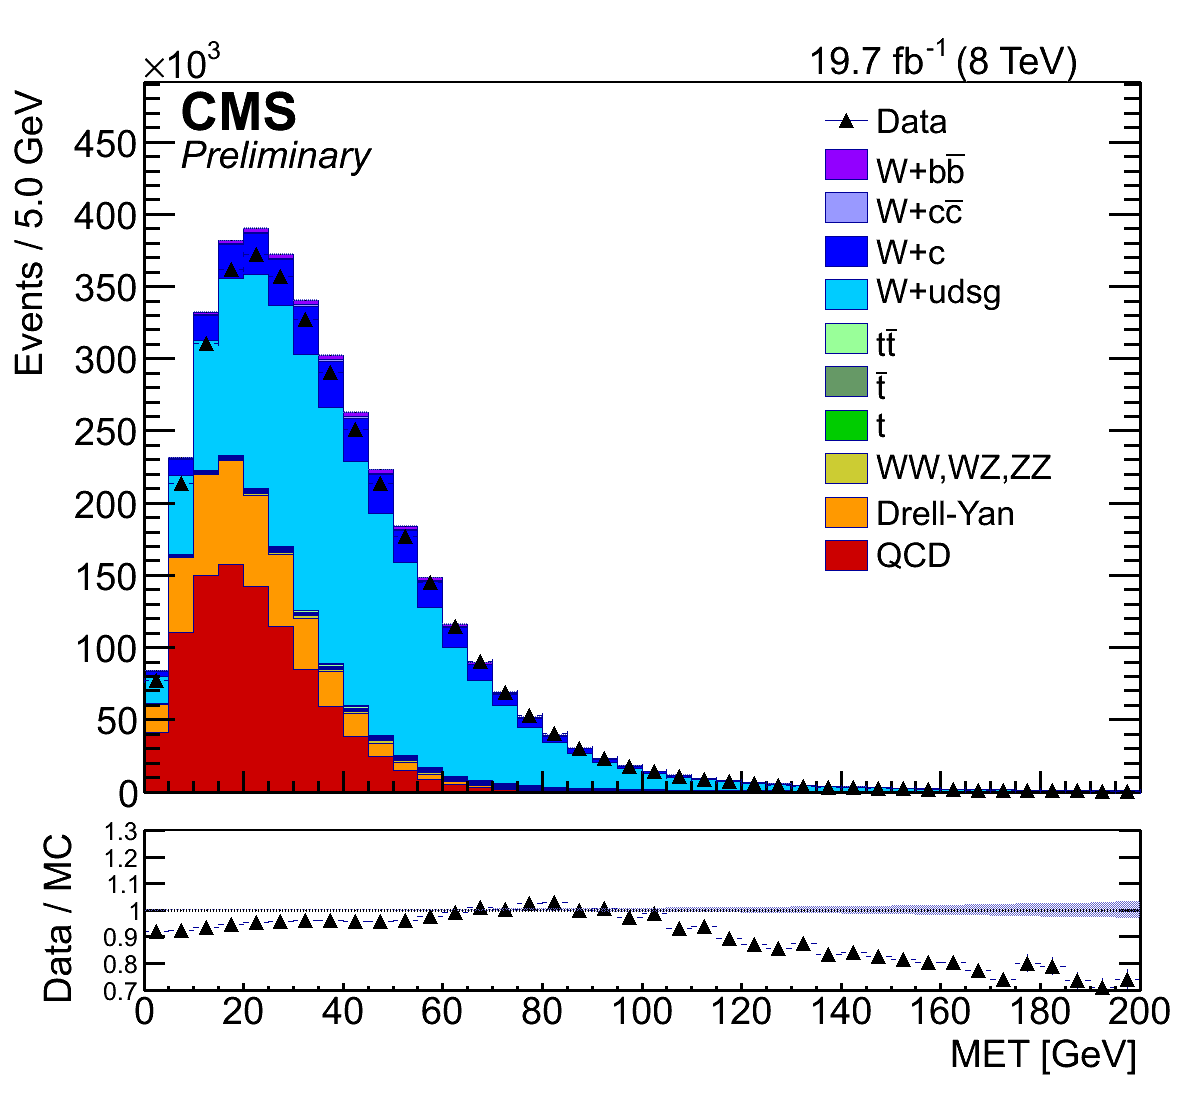
\includegraphics[width=0.4\textwidth]{/Users/rhombus/CMS/Thesis/thesis/pdfs/wbbxc/wjj/Histograms_wjj_met_ele.png} \\
 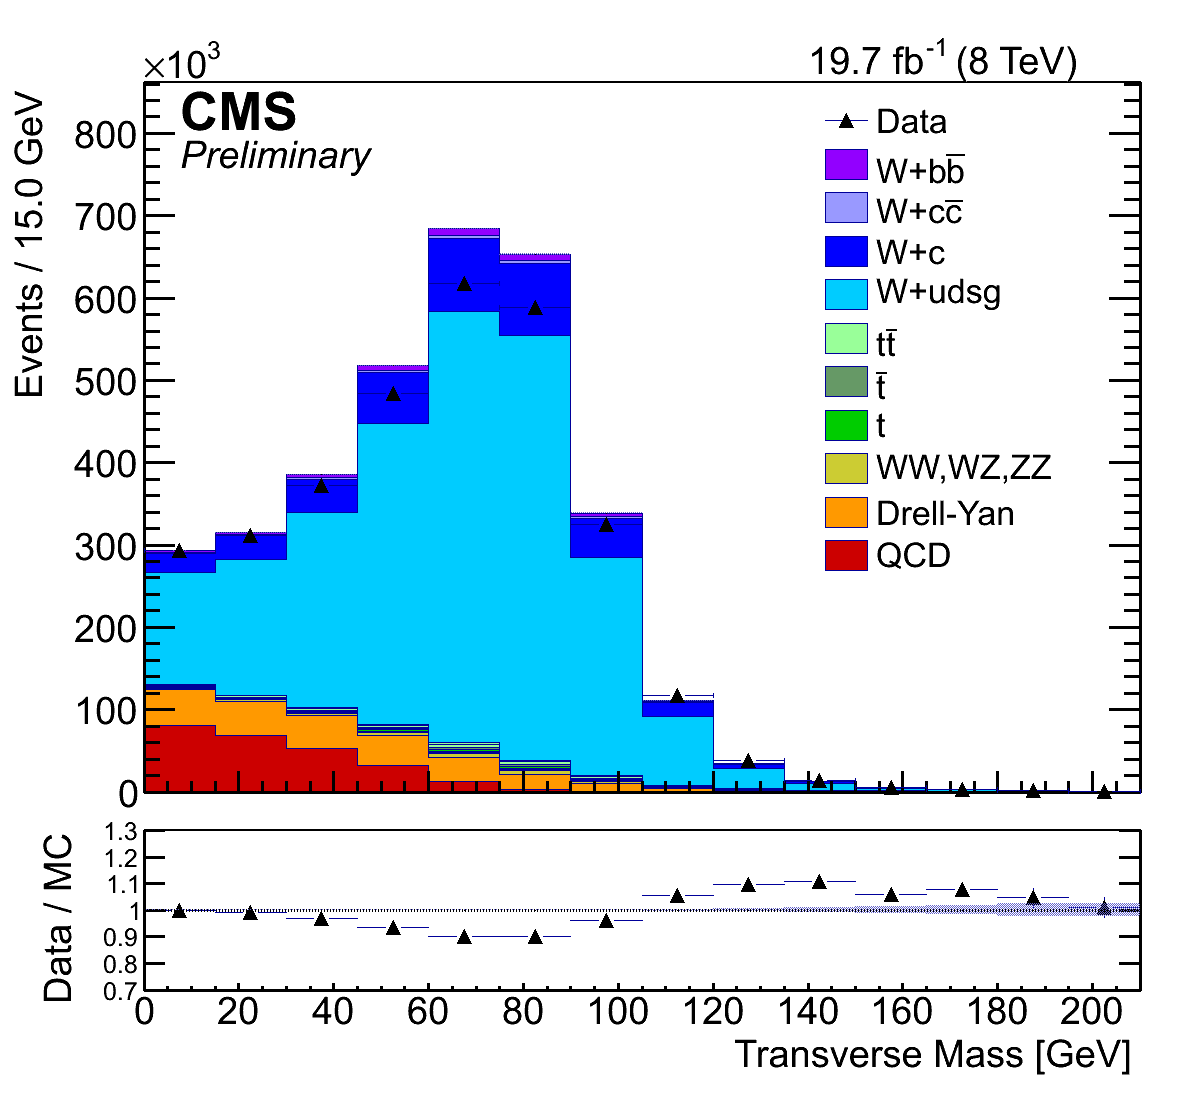
\includegraphics[width=0.4\textwidth]{/Users/rhombus/CMS/Thesis/thesis/pdfs/wbbxc/wjj/Histograms_wjj_mt_mu.png}  & 
 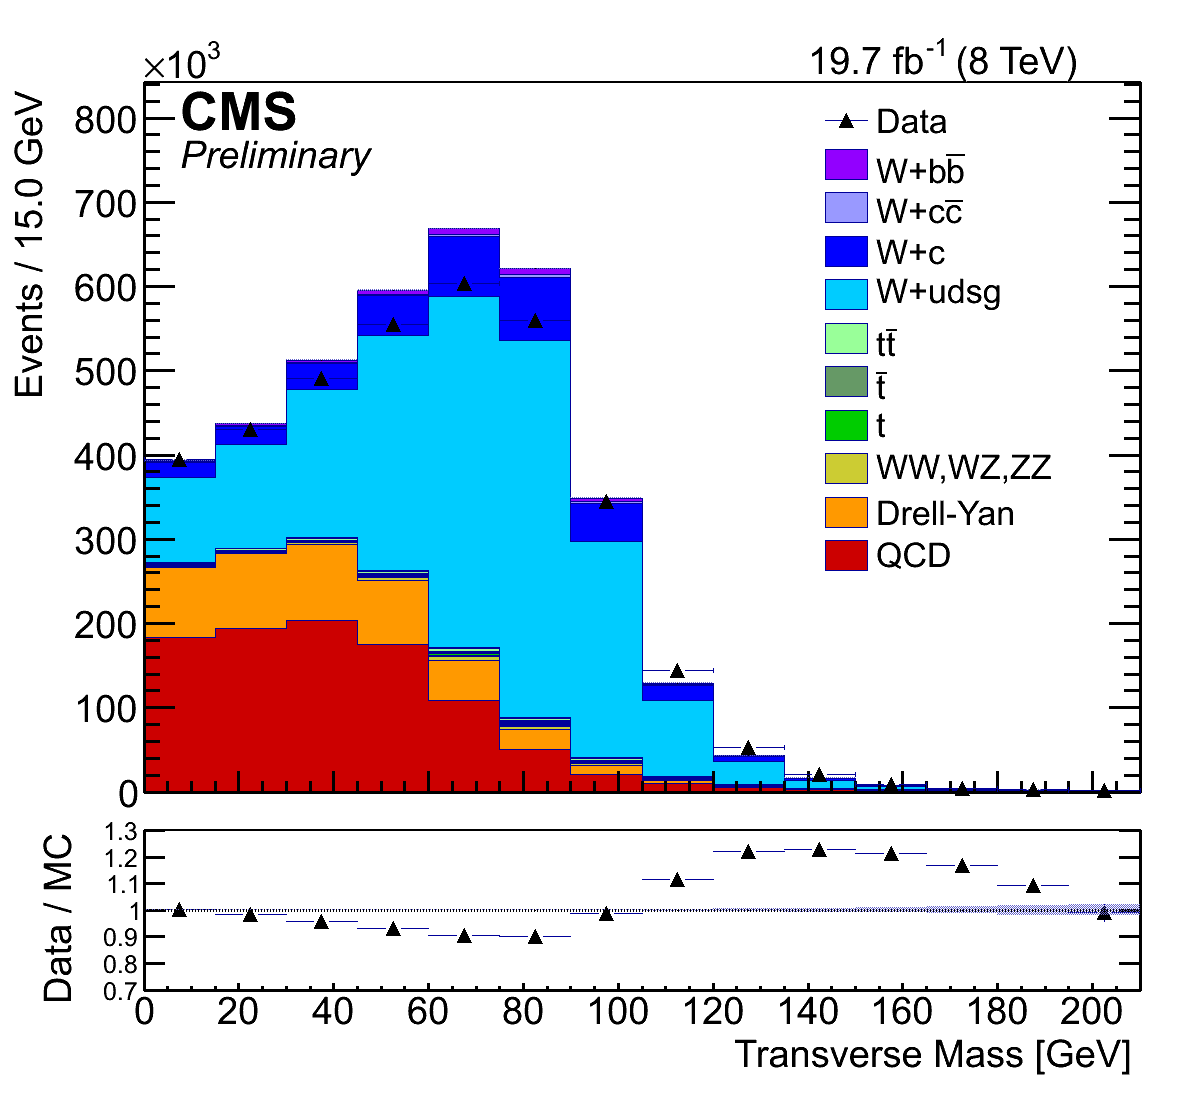
\includegraphics[width=0.4\textwidth]{/Users/rhombus/CMS/Thesis/thesis/pdfs/wbbxc/wjj/Histograms_wjj_mt_ele.png} 
\end{tabular}
\end{centering}
    \label{fig:wjj_plots}
\end{figure}

The process $\ppwb$ with a single $b$ quark
 produced is CKM suppressed by two generations
 if light quarks are interacting.
The process $\ppwc$ is only suppressed by one
 generation but is still found to contribute
 negligible rate in the signal region due to
 the requirement of a second $b$ tag along
 with a veto on a third jet.
A second jet can be added to $ppwc$ via ISR or FSR,
 and light quarks require less energy to produce
 than heavy quarks, making them more probable.
Therefore, the dominant contribution to 
 $ppwc$ in the signal region comes from the 
 mistag of a $c$ jet for a $b$ jet, along with 
 the misidentification of an ISR/FSR light jet.
However, the contribution to events in the signal region
 from high energy \gcc is not negligable and
 moreover these events have kinematics closely related 
 to that of the signal. 

\subsection{Single top backgrounds}
\label{section:topbackgrounds}

\begin{figure}
\caption[Diagram for single top $t$-channel control region]
{
Below is the diagram for the process attempting
 to be isolated in the single top $t$-channel 
 control region.
}
\center
 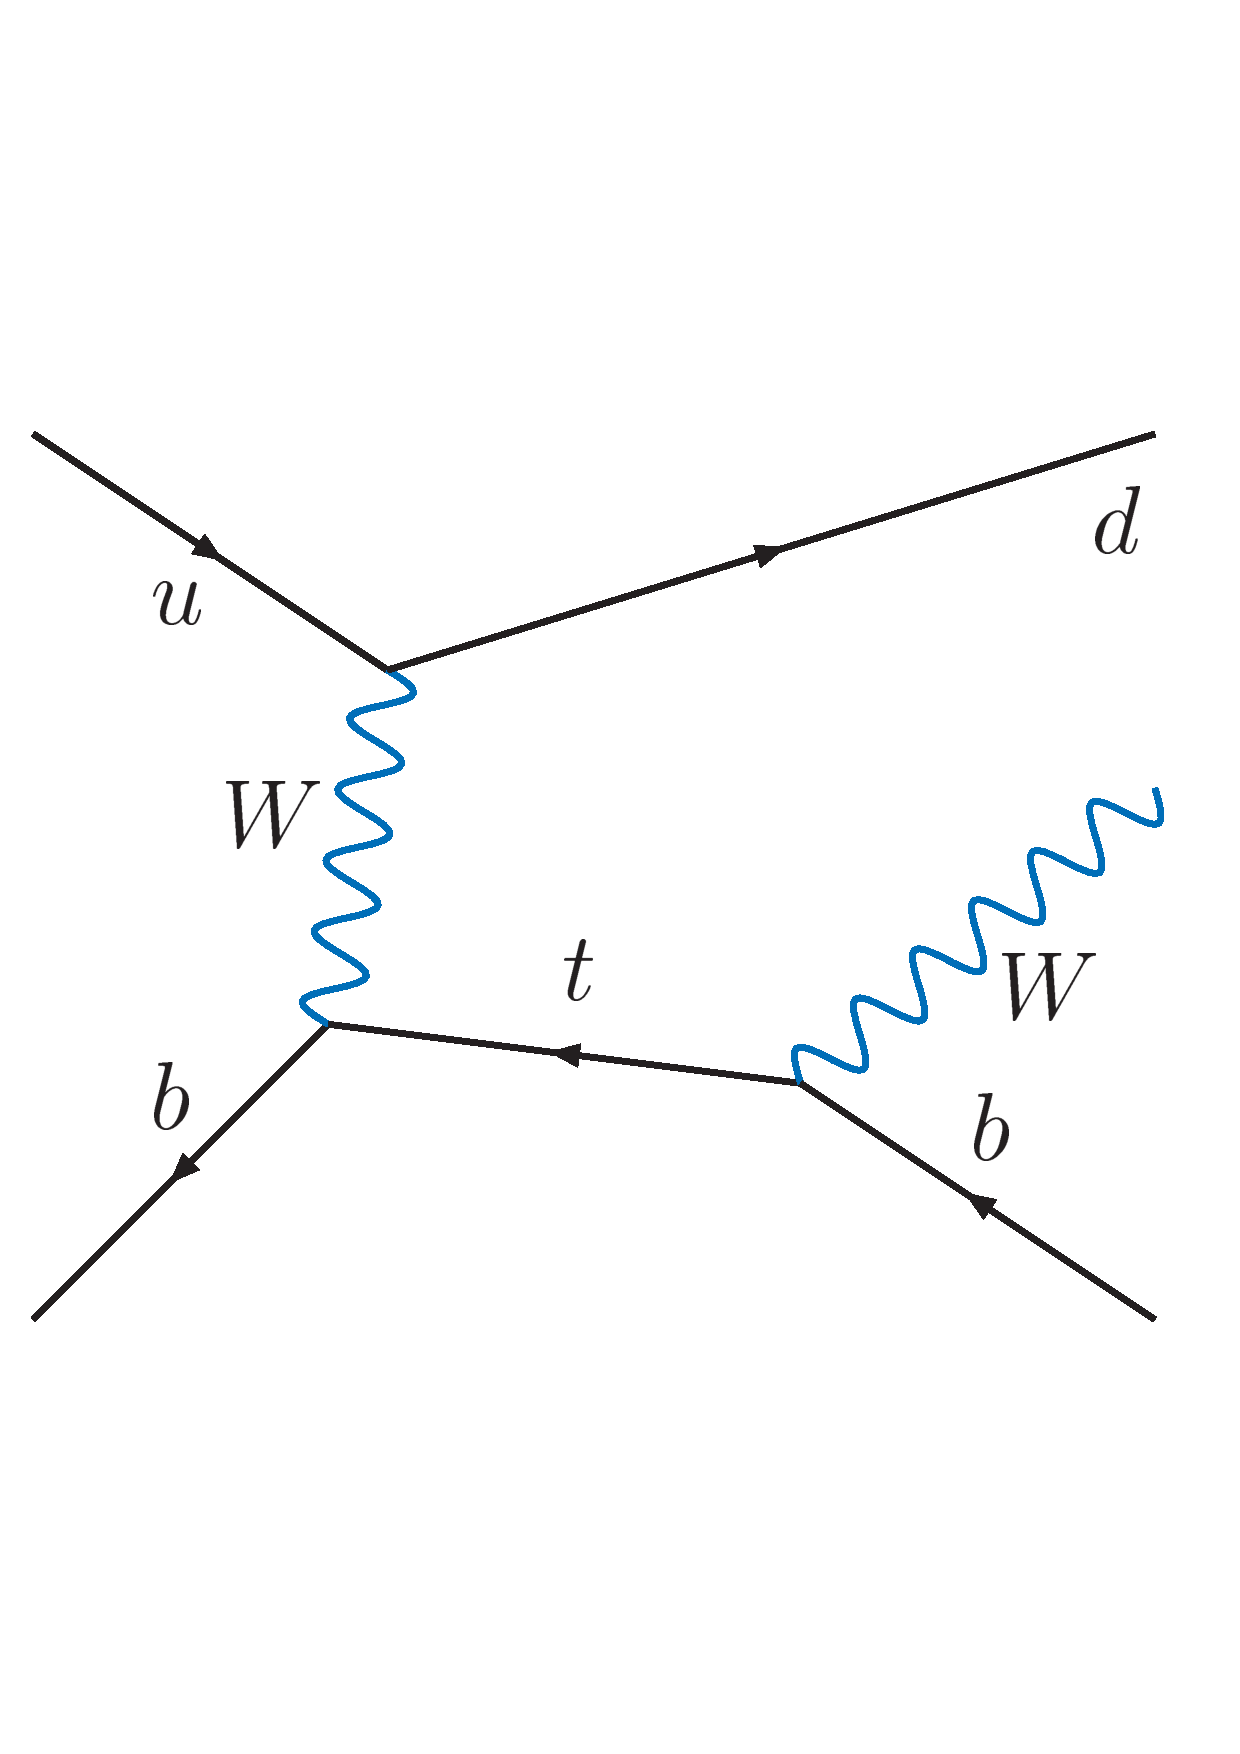
\includegraphics[width=0.4\textwidth]{/Users/rhombus/CMS/Thesis/thesis/pdfs/feyn/st_tchannel.pdf}
\label{fig:feynstt}
\end{figure}

The single top $t$-channel control region is defined by the signal selection requirements
 without the third and forward jet vetos, and
 with the leading jet required to be central
 ($|\eta|<2.4$) and tightly $b$-tagged,
 while the subleading jet has no $b$ requirement and must fall within
 $2.4<|\eta|<5.0$.
The reasons for these selections are based on examination
 of Figure~\ref{fig:feynstt}.
The $b$ quark is a product of the $t$ decay and is recoiling
 against a $W$, making it a high-\pt jet.
The other jet comes from an initial state
 quark that exchanges a $W$ and recoils against the  $t$.
Because it is the product of an initial state quark which
 is most likely to be light,
 the final state jet is also most likely to be light.
The fact that it is recoiling against the much more massive $t$
 means that it is likely be forward by conservation of momentum.
As can be seen in Figure \ref{fig:prefit_stt}, there are many 
 backgrounds contaminating the purity of this phase space,
 but agreement between data and simulation is on the order of 5-10\%.

\begin{figure}
      \caption[Single-top control region for the \wbb measurement]{The single top control region is defined by one $b$-tagged central jet and one forward jet.
      Shown above are distributions in the single top control region.
       Left plots are in the muon decay channel and right
        plots are in the electron decay channel.
      }
\begin{centering}
\begin{tabular}{cc}
 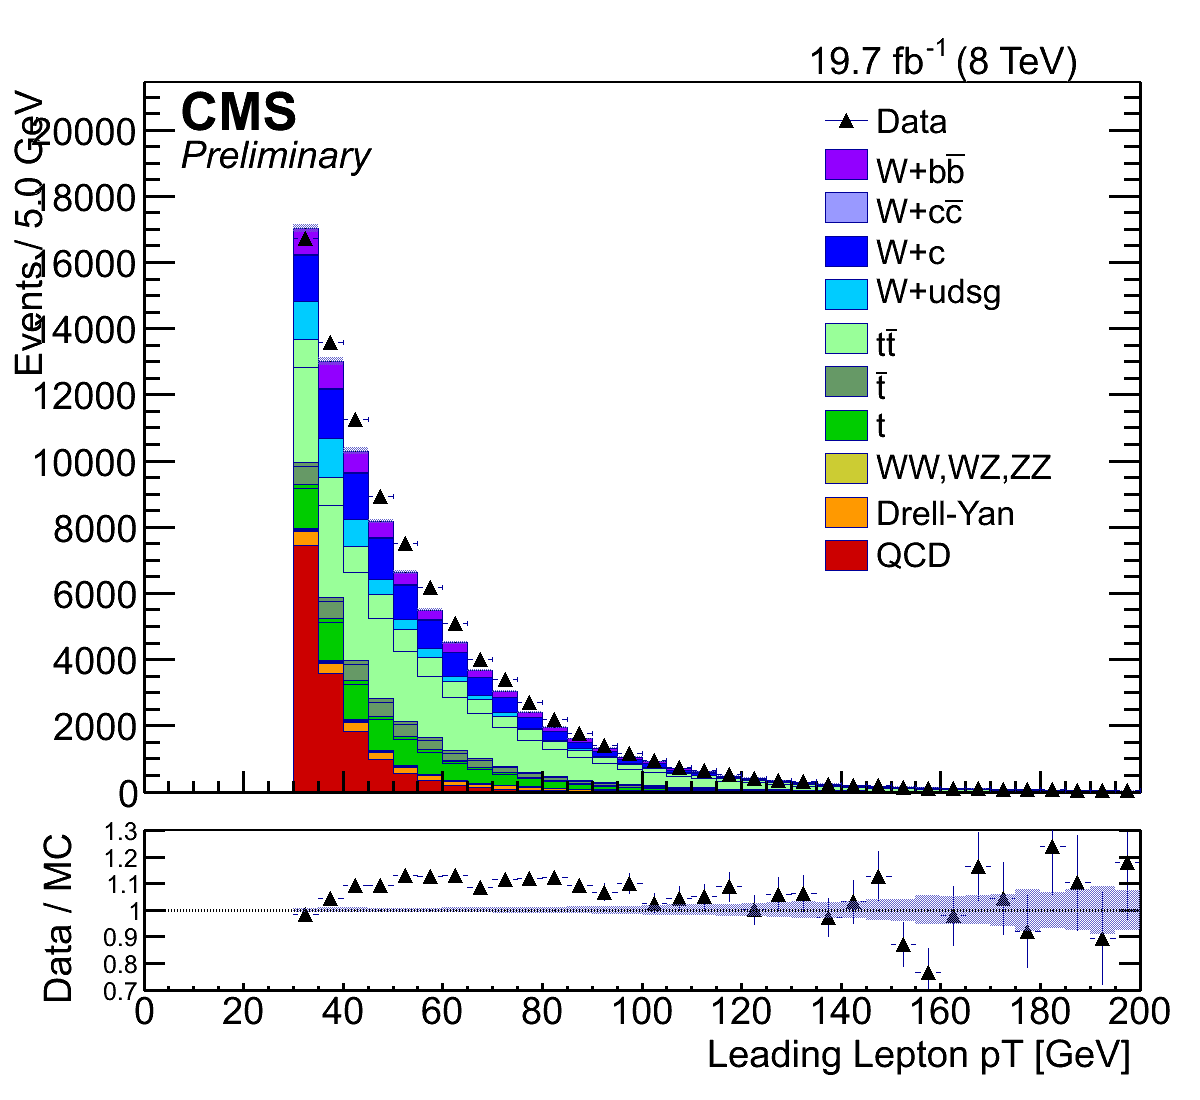
\includegraphics[width=0.4\textwidth]{/Users/rhombus/CMS/Thesis/thesis/pdfs/wbbxc/stt/Histograms_stt_goodLep_pt_mu.png} &
 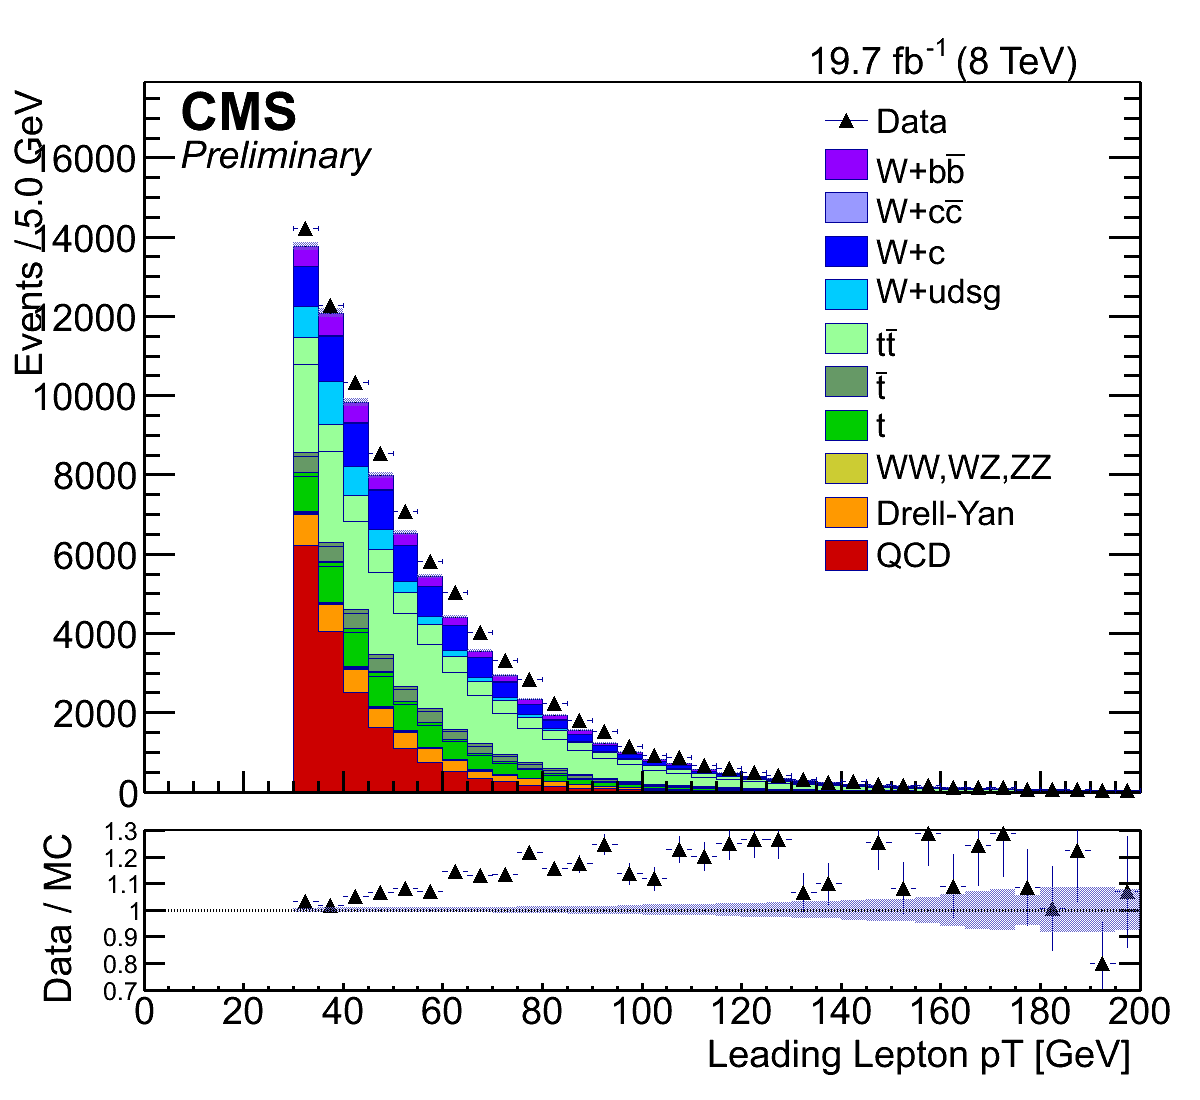
\includegraphics[width=0.4\textwidth]{/Users/rhombus/CMS/Thesis/thesis/pdfs/wbbxc/stt/Histograms_stt_goodLep_pt_ele.png} \\
 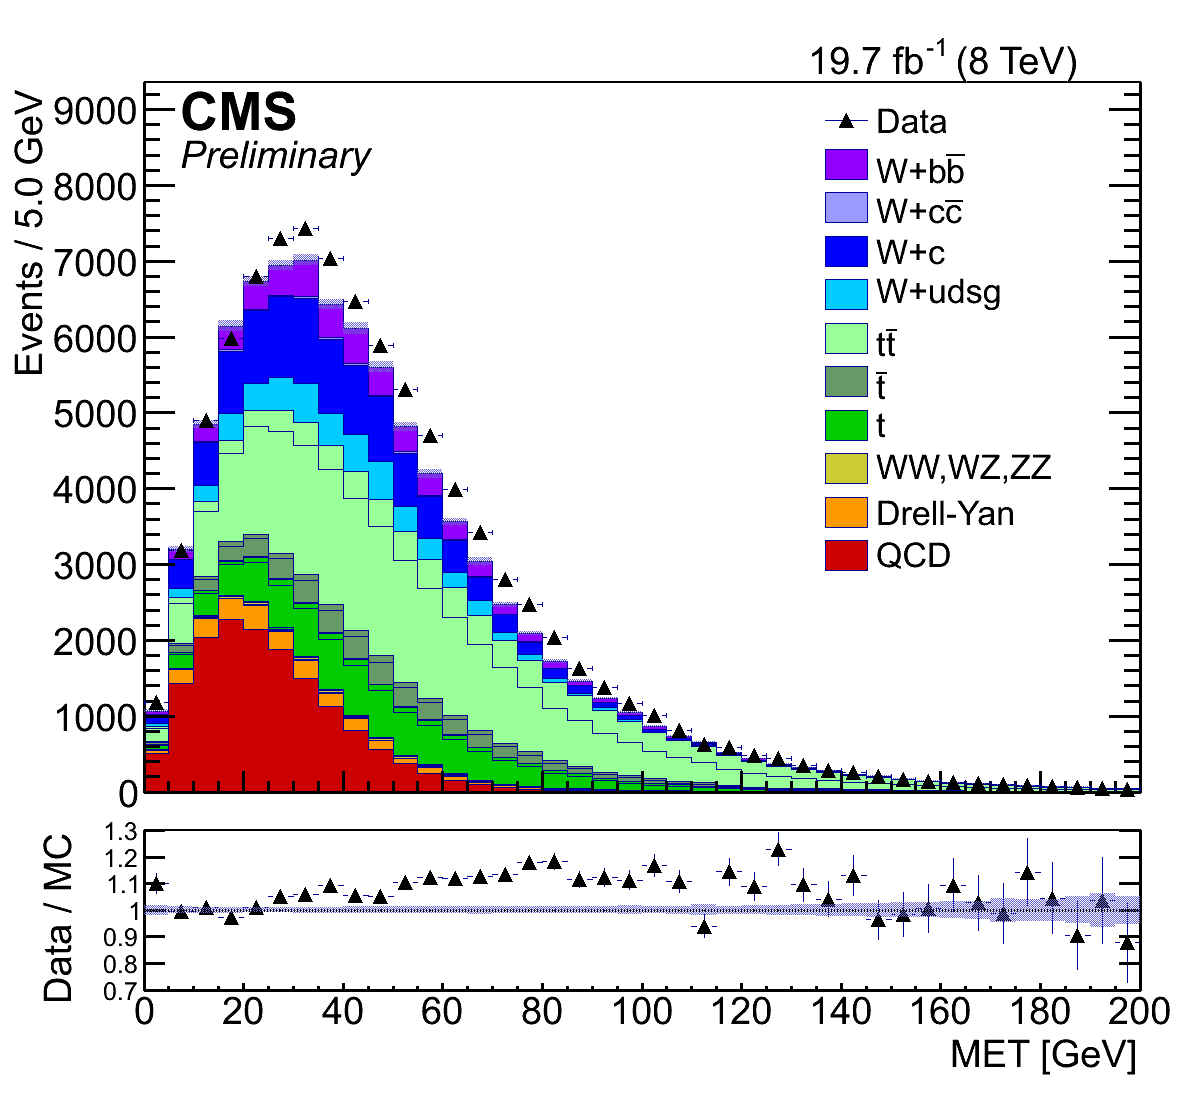
\includegraphics[width=0.4\textwidth]{/Users/rhombus/CMS/Thesis/thesis/pdfs/wbbxc/stt/Histograms_stt_met_mu.png} & 
 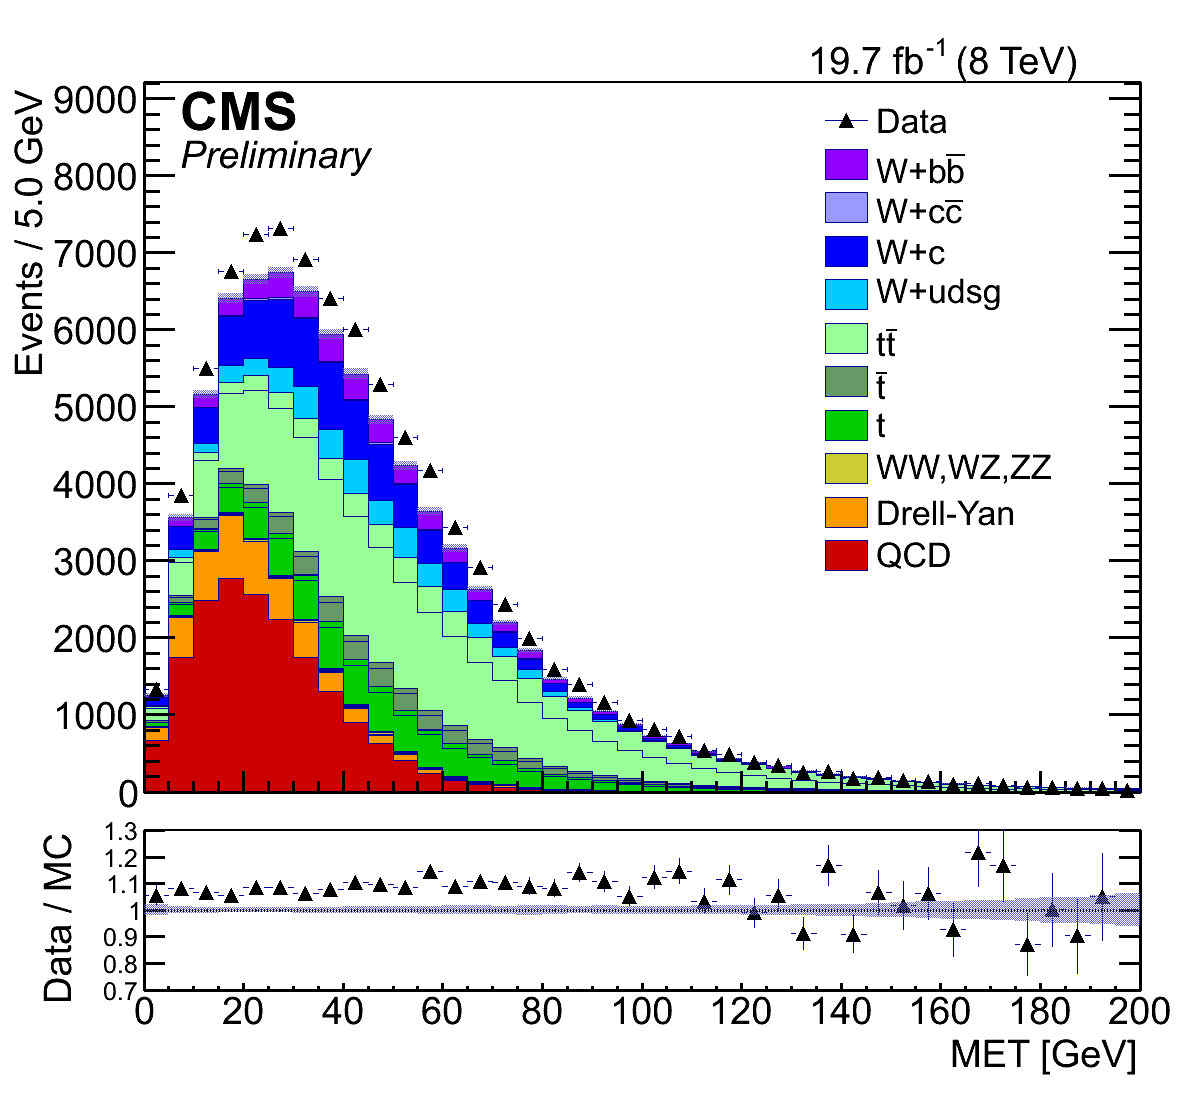
\includegraphics[width=0.4\textwidth]{/Users/rhombus/CMS/Thesis/thesis/pdfs/wbbxc/stt/Histograms_stt_met_ele.png} \\
 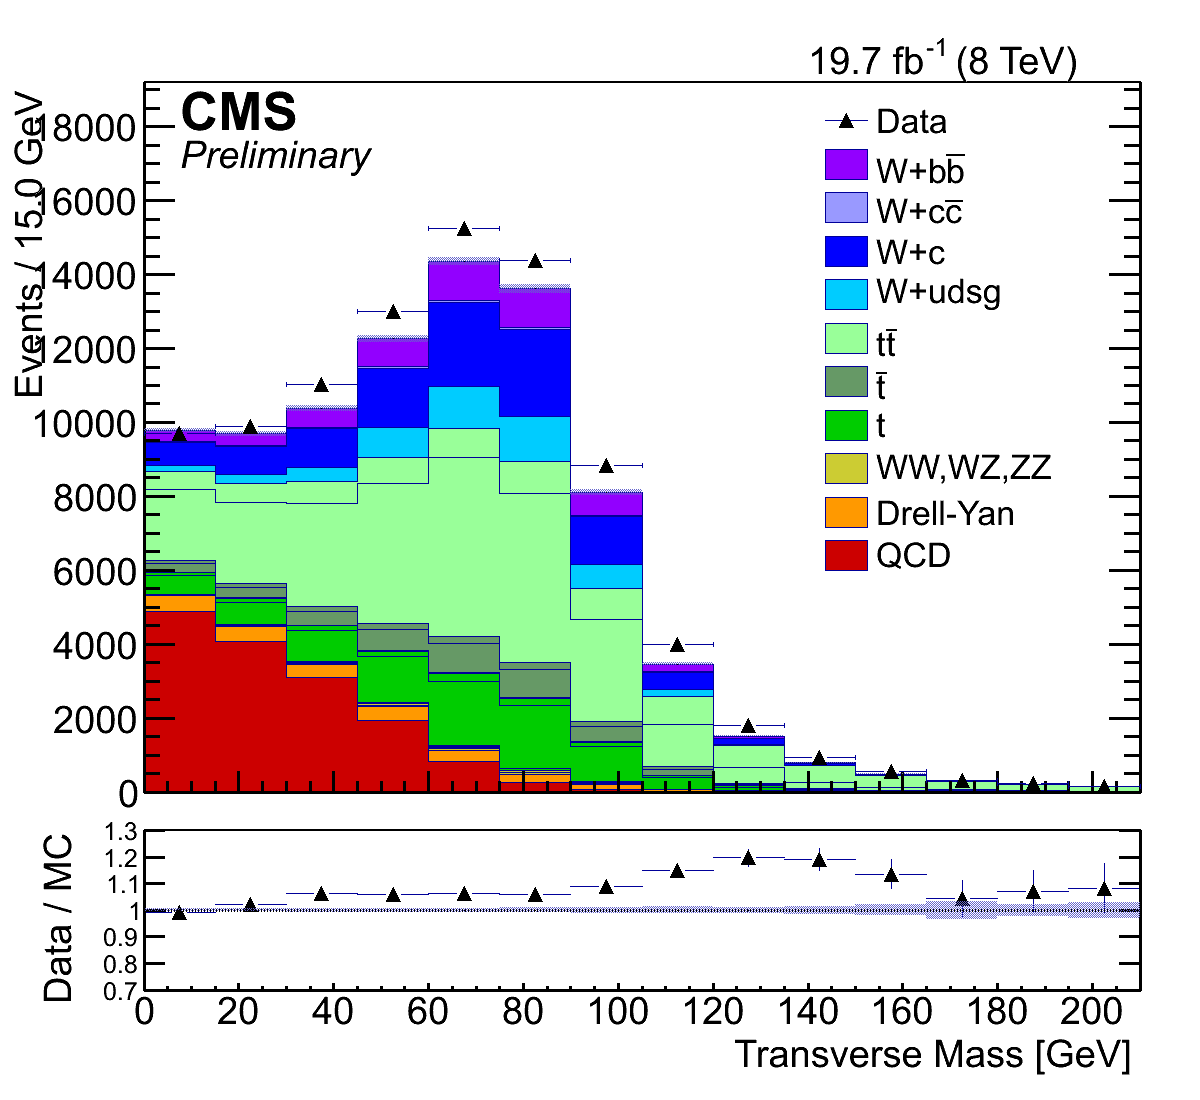
\includegraphics[width=0.4\textwidth]{/Users/rhombus/CMS/Thesis/thesis/pdfs/wbbxc/stt/Histograms_stt_mt_mu.png} & 
 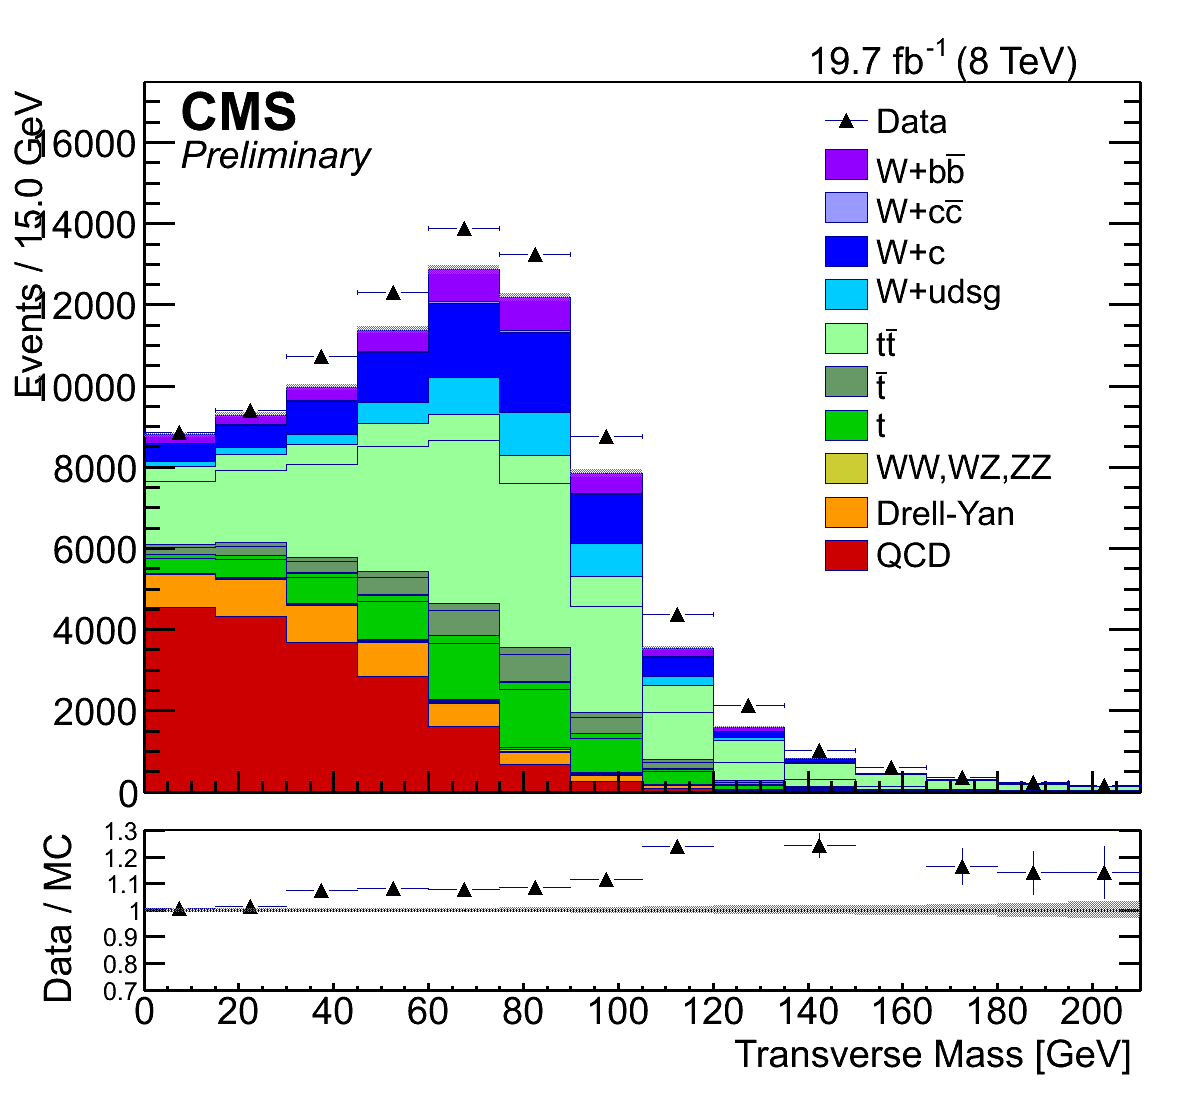
\includegraphics[width=0.4\textwidth]{/Users/rhombus/CMS/Thesis/thesis/pdfs/wbbxc/stt/Histograms_stt_mt_ele.png}
\end{tabular}
\end{centering}
      \label{fig:prefit_stt}
\end{figure}


\subsection[\zll backgrounds]{$\boldsymbol{\zll}$ backgrounds}

The Drell-Yan backround is validated in a control region where the $\wbb$
 selection requirements are applied, but the lepton veto 
 is inverted, requiring two isolated, same-flavor leptons
 which are presumed to be the decay products of the $Z$ boson.
This is referred to as the $\zbb$ region and distributions
 of the mass and transverse momentum of the dilepton pair is
 shown in Figure \ref{fig:prefit_dybb}.
Contamination from \ttbar is evident. 
A cleaner Drell-Yan phase space is found by requiring exactly two jets
 but placing no $b$ tag requirement and is referred to as $\zjj$.
Figure \ref{fig:prefit_dyjj} shows the same distributions as
 Figure \ref{fig:prefit_dybb} in this phase space.
%More cross checks on Drell-Yan are shown in Appendix \ref{sec:dycrosscheck}.

\begin{figure}
      \caption[\zbb control region for the \wbb analysis]{ Above are distributions of the mass and
        transverse momentum of the dilepton pair in the
        $\zbb$ phase space.
       Left plots are in the muon decay channel and right
        plots are in the electron decay channel.
      }
      \center
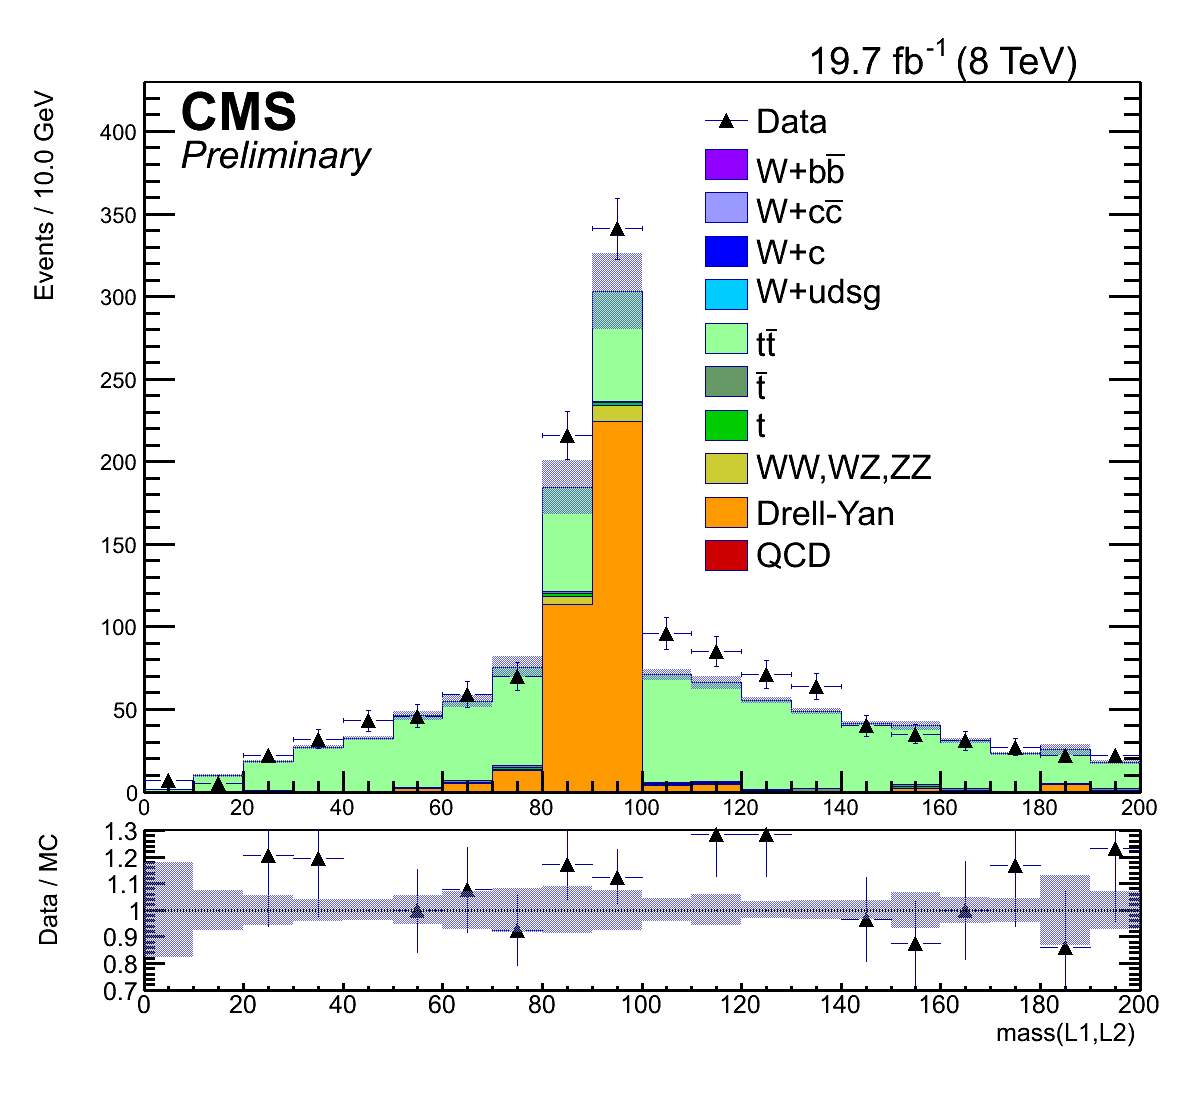
\includegraphics[width=0.4\textwidth]{/Users/rhombus/CMS/Thesis/thesis/pdfs/wbbxc/dy/Histograms_e2CJ_xFJ_tB2_goodL1L2_mass_mu.png}
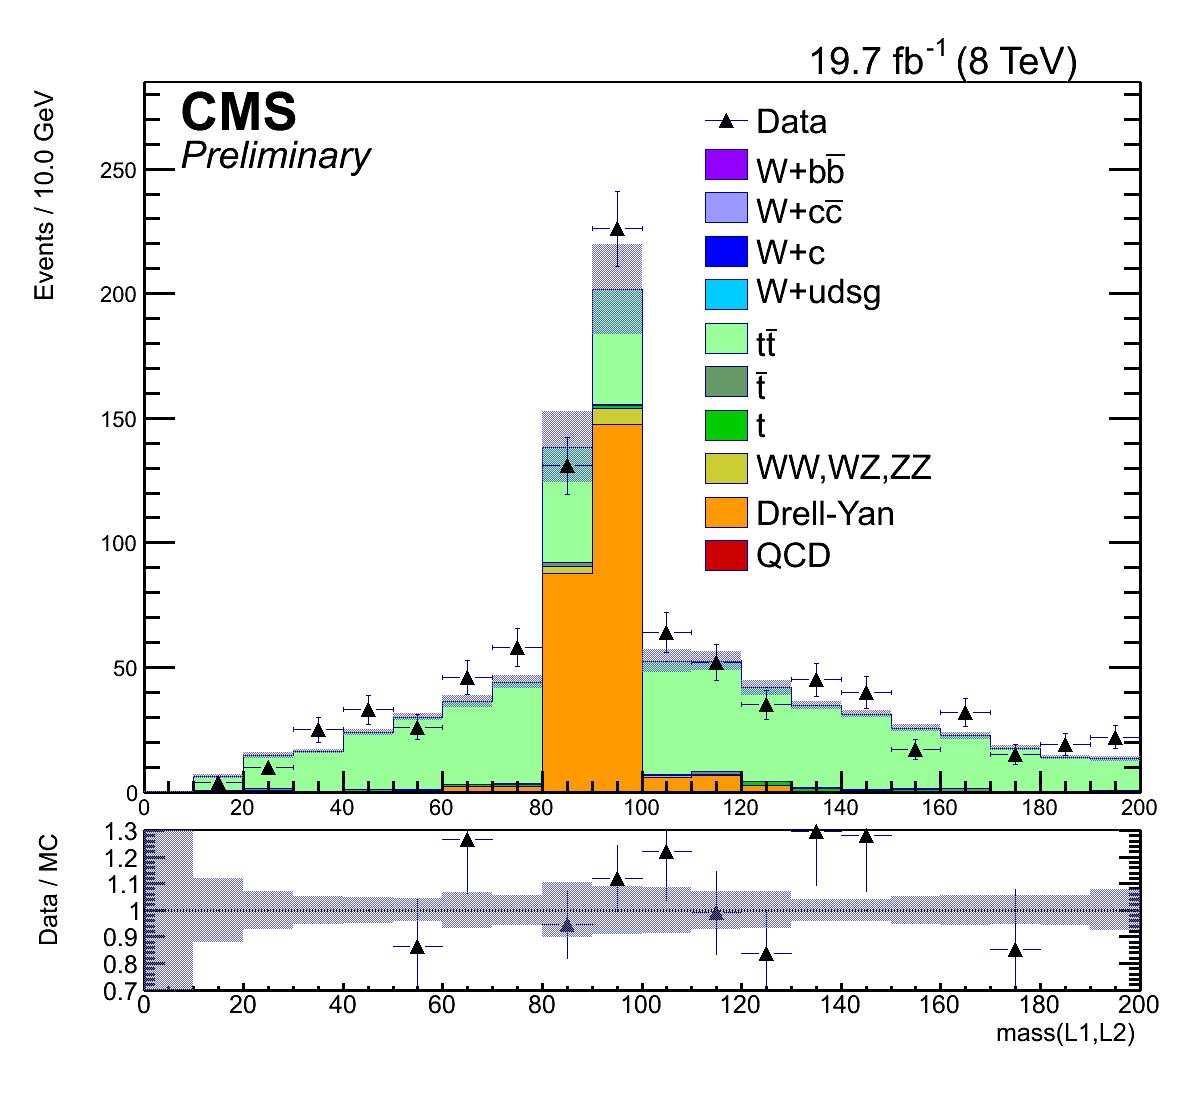
\includegraphics[width=0.4\textwidth]{/Users/rhombus/CMS/Thesis/thesis/pdfs/wbbxc/dy/Histograms_e2CJ_xFJ_tB2_goodL1L2_mass_ele.png}
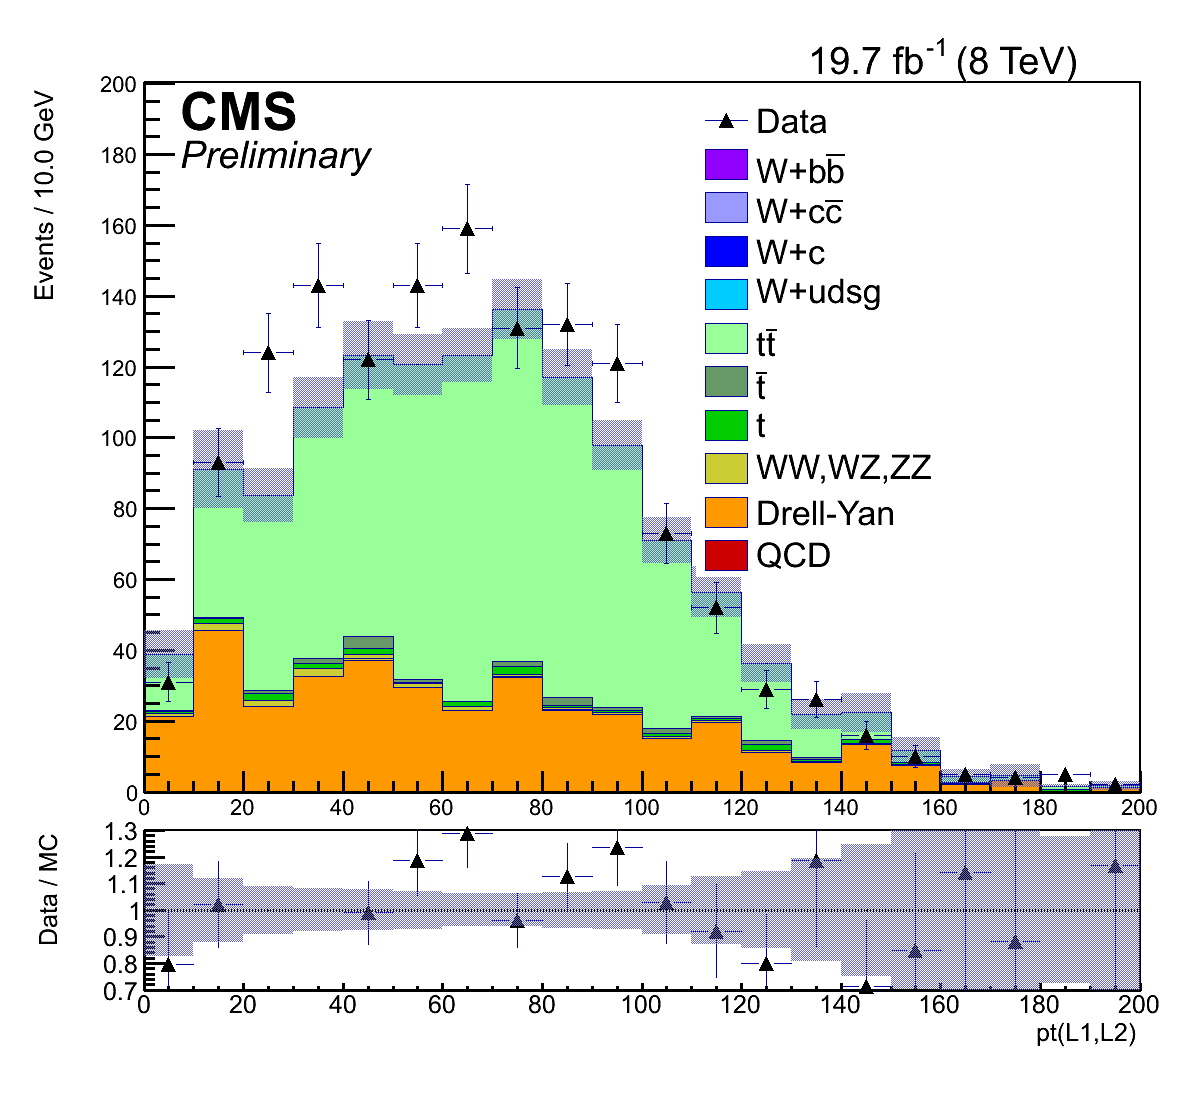
\includegraphics[width=0.4\textwidth]{/Users/rhombus/CMS/Thesis/thesis/pdfs/wbbxc/dy/Histograms_e2CJ_xFJ_tB2_goodL1L2_pt_mu.png}
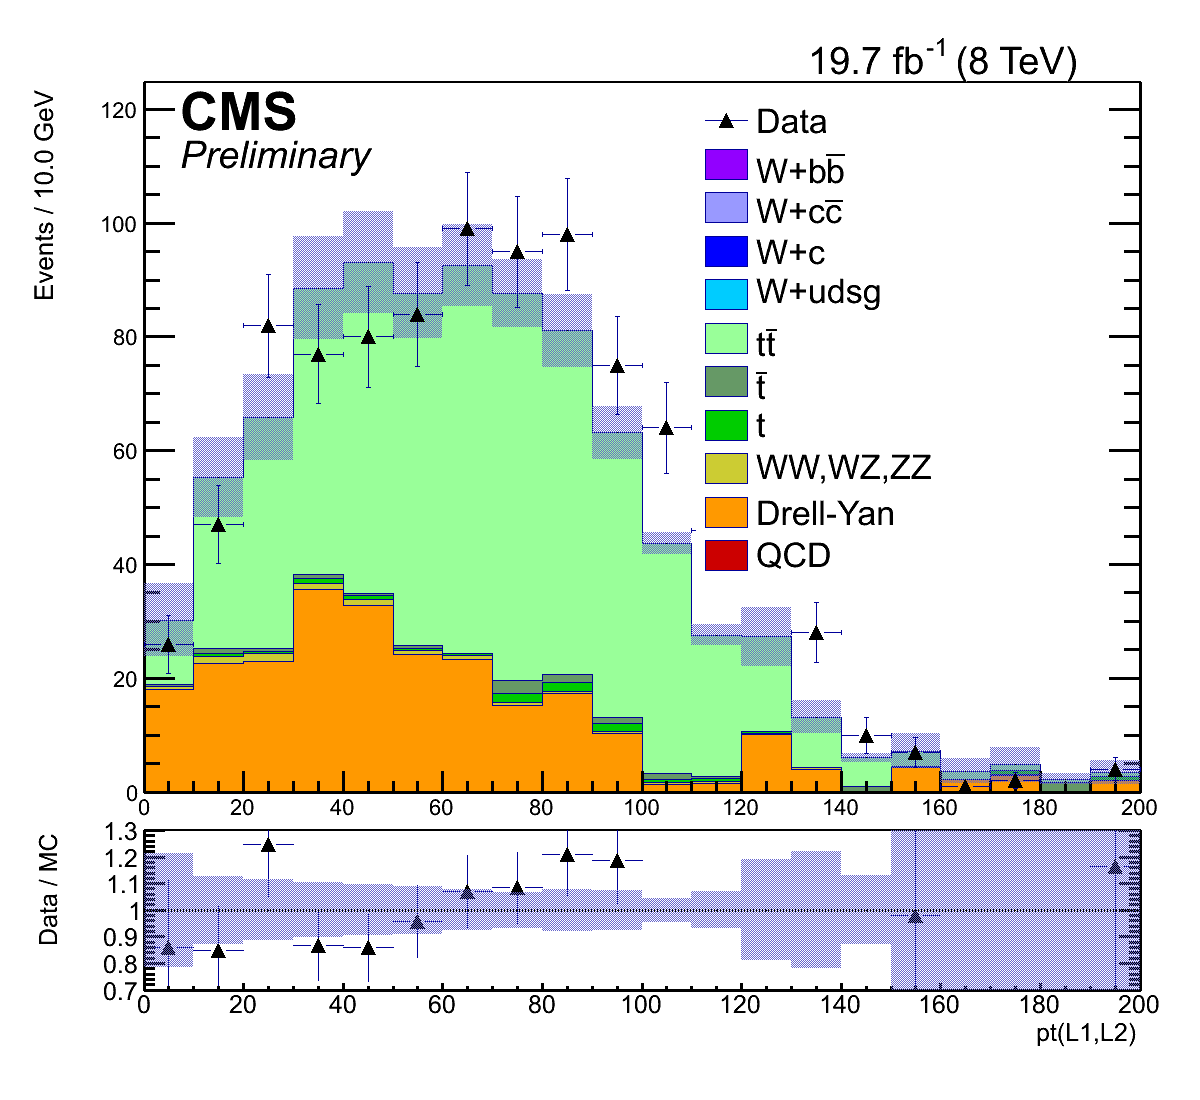
\includegraphics[width=0.4\textwidth]{/Users/rhombus/CMS/Thesis/thesis/pdfs/wbbxc/dy/Histograms_e2CJ_xFJ_tB2_goodL1L2_pt_ele.png}
      \label{fig:prefit_dybb}
\end{figure}

\begin{figure}
      \caption[\zjj control region for the \wbb measurement]{ Above are distributions of the mass and
        transverse momentum of the dilepton pair in the
        $\zjj$ phase space.
       Left plots are in the muon decay channel and right
        plots are in the electron decay channel.
      }
      \center
 \subfloat[]{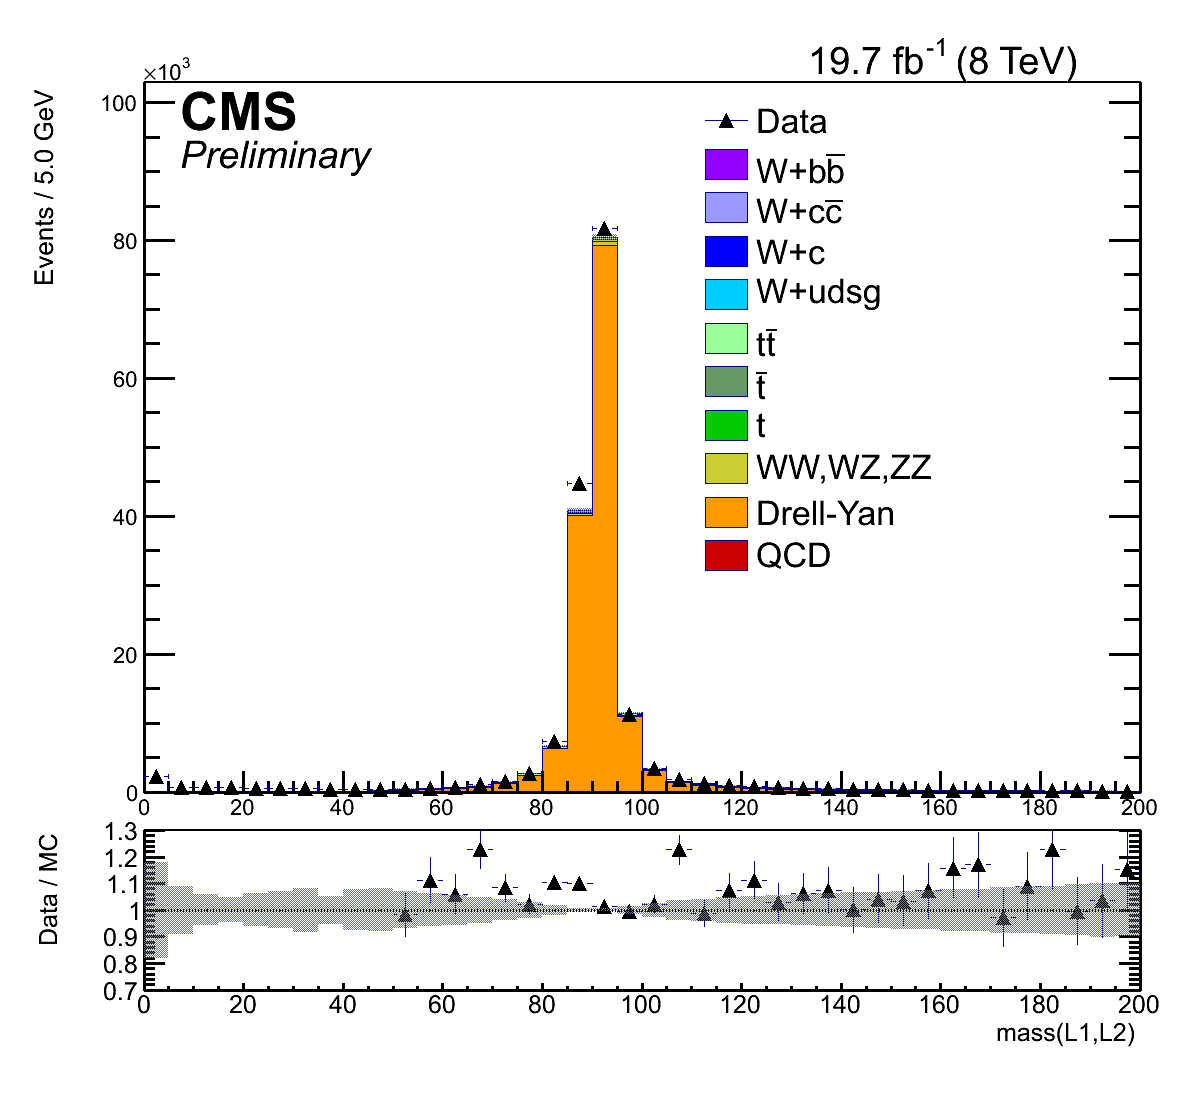
\includegraphics[width=0.4\textwidth]{/Users/rhombus/CMS/Thesis/thesis/pdfs/wbbxc/dy/Histograms_e2CJ_xFJ_goodL1L2_mass_mu.png}}
 \subfloat[]{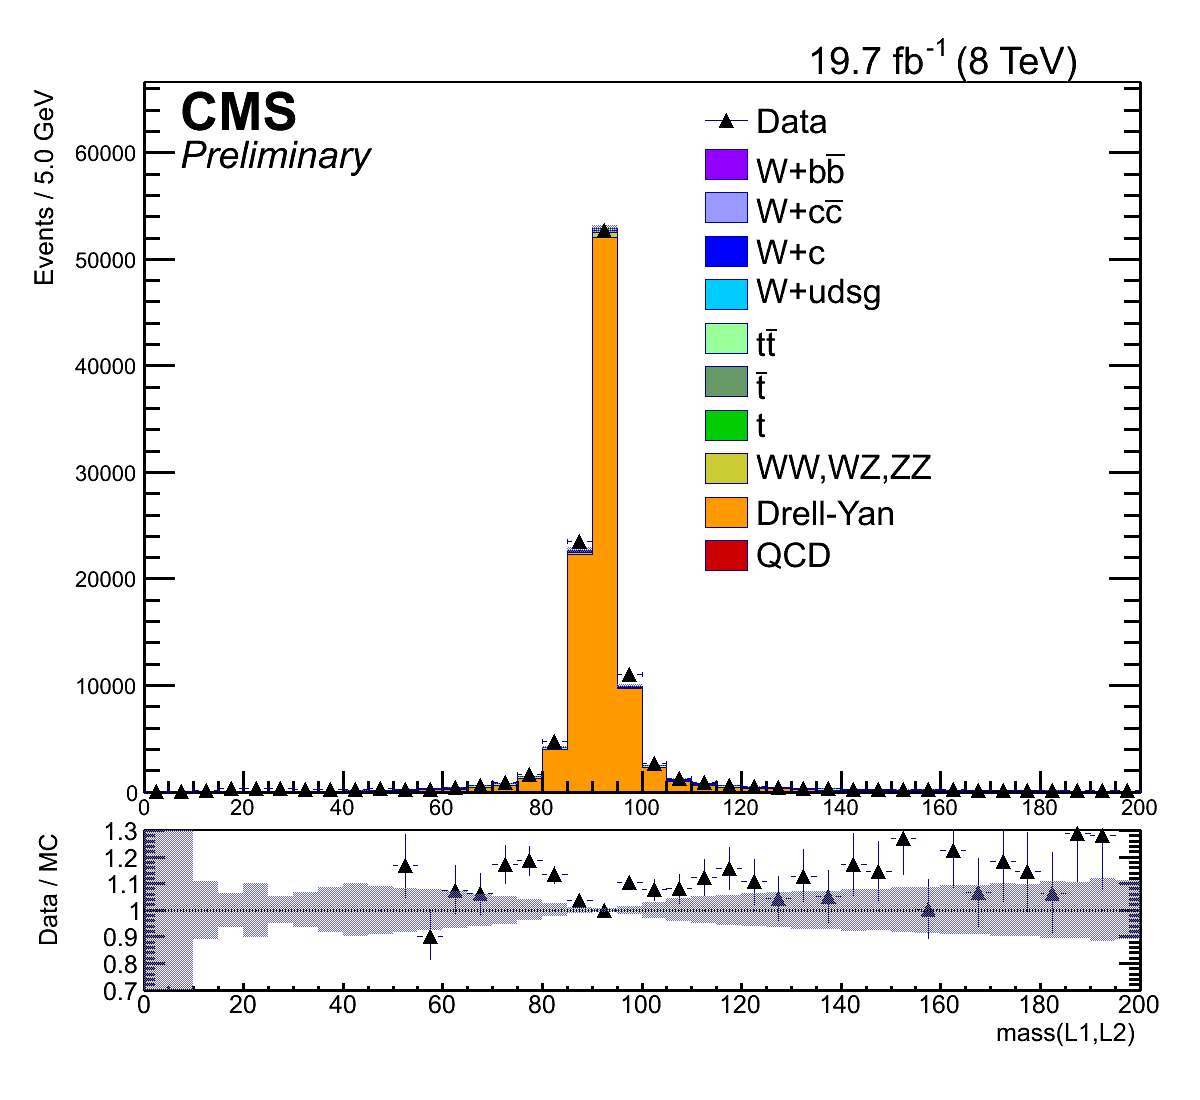
\includegraphics[width=0.4\textwidth]{/Users/rhombus/CMS/Thesis/thesis/pdfs/wbbxc/dy/Histograms_e2CJ_xFJ_goodL1L2_mass_ele.png}}
  \\
 \subfloat[]{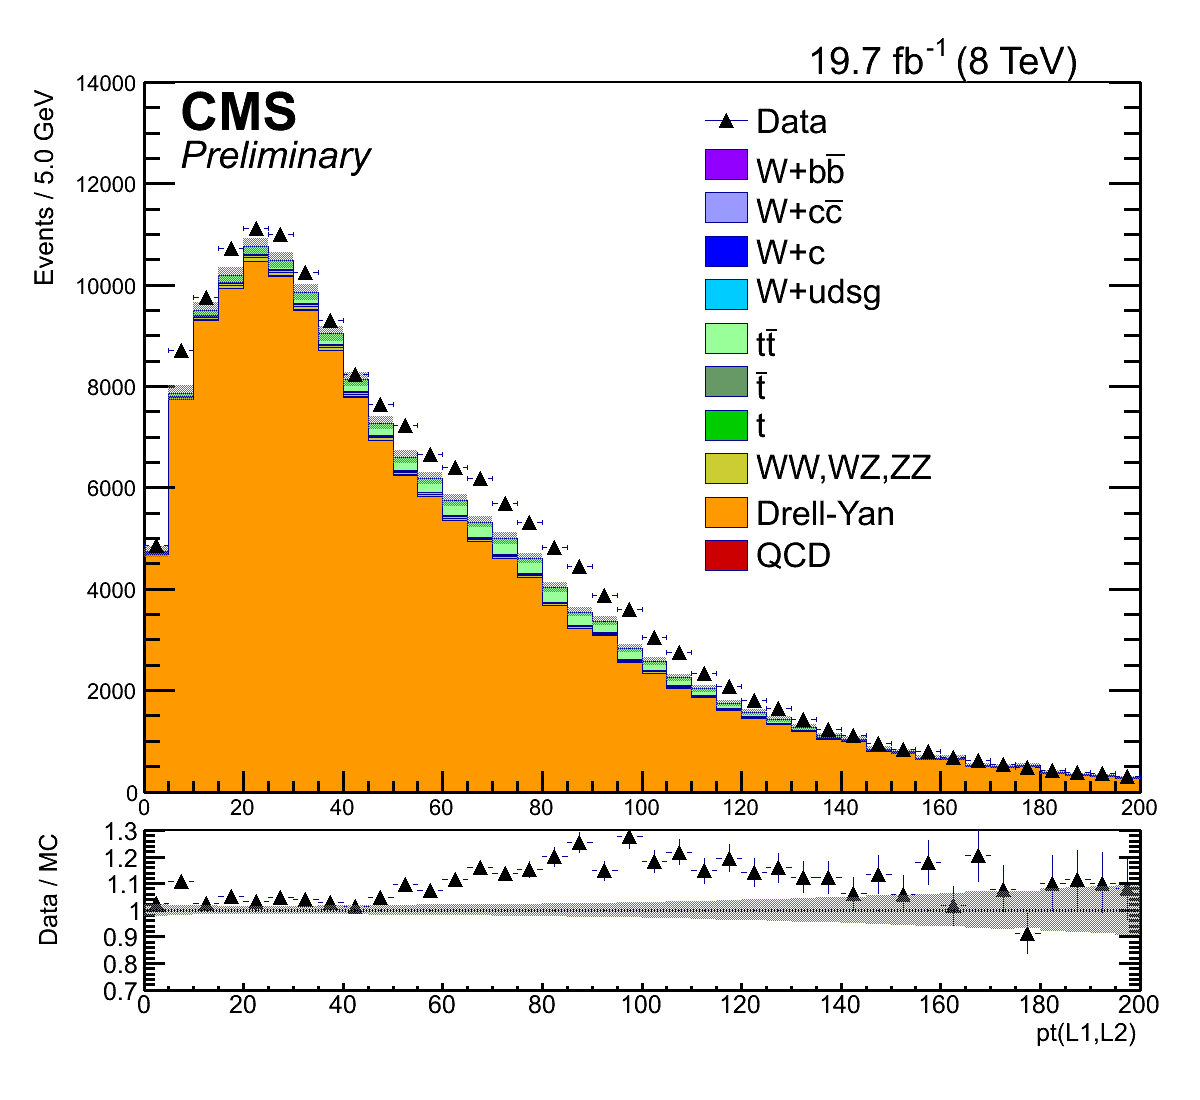
\includegraphics[width=0.4\textwidth]{/Users/rhombus/CMS/Thesis/thesis/pdfs/wbbxc/dy/Histograms_e2CJ_xFJ_goodL1L2_pt_mu.png}}
 \subfloat[]{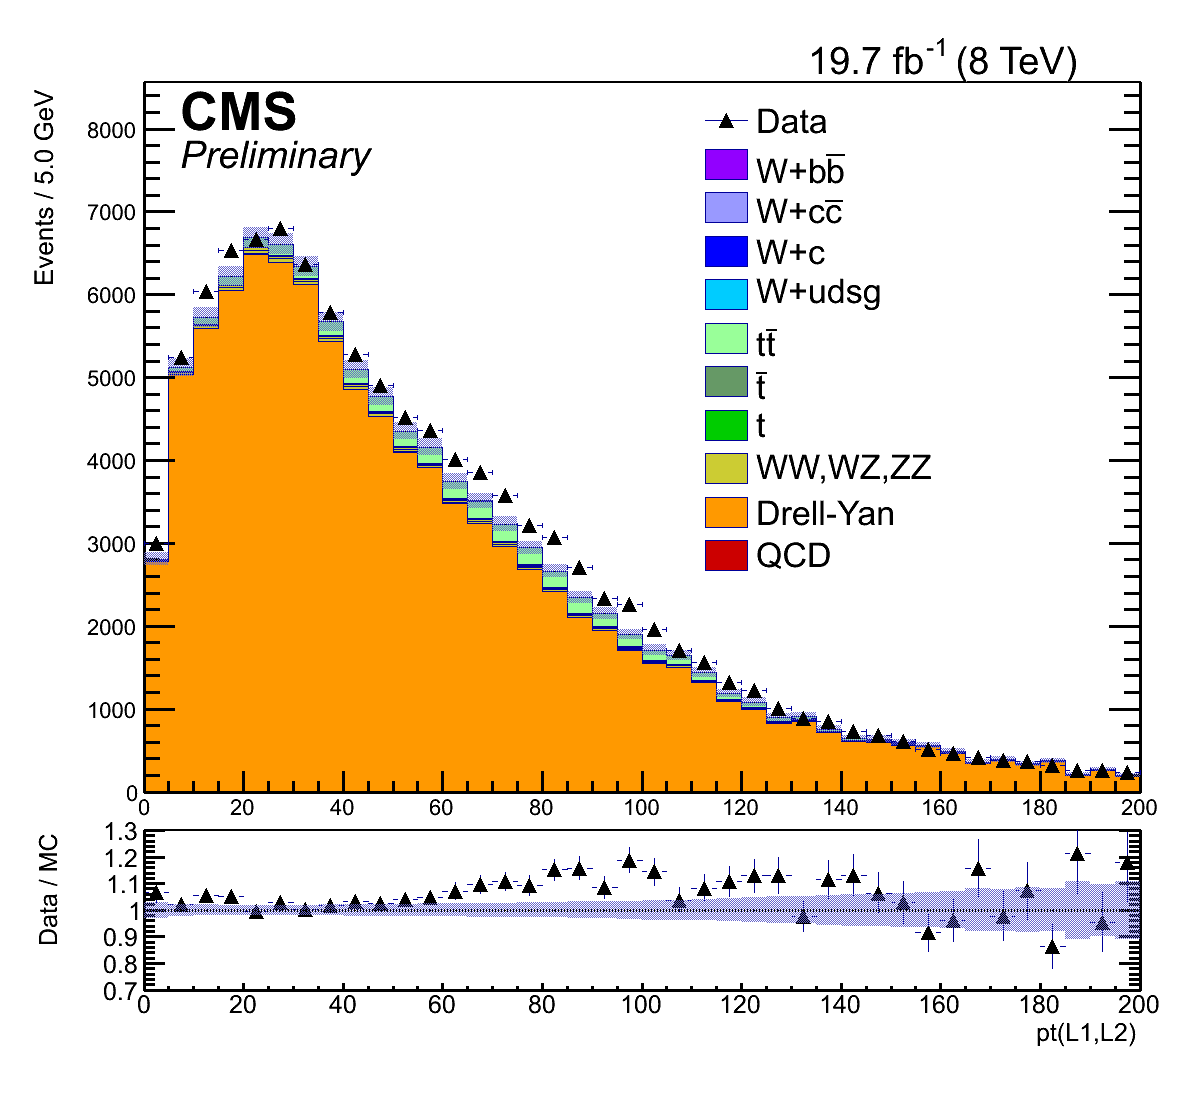
\includegraphics[width=0.4\textwidth]{/Users/rhombus/CMS/Thesis/thesis/pdfs/wbbxc/dy/Histograms_e2CJ_xFJ_goodL1L2_pt_ele.png}}
  \\
      \label{fig:prefit_dyjj}
\end{figure}


\section{Analysis Strategy}\label{sec:wbb_analysisstrategy}
The \wbb yield is measured using a likelihood fit 
 to the $\mt$ distribution in the signal region.
With the exception of QCD processes,
 the initial shapes and normalizations of all contributions
 in the fit are taken from simulation.
Consequently, it is important
 to verify that 
 the simulation describes the data.
The dominant background in the signal region arises 
 from the $\ttbar$ process.
The data and simulation
 are thus compared in two $\ttbar$-dominated control regions:
 one characterized by a pair of opposite flavor leptons,
 and the other by the presence of three or more jets.
The simulation is reweighted to describe the data in the control regions
 and then is used to predict the $\mt$ distributions
 in the signal region.

The signal region requires a muon (electron)
 with {$\pt > 30$} GeV,
 {$|\eta| < 2.1$}, and satisfying {$I < 0.12~(0.10)$}.
 %as defined in Eq. \ref{eq:iso}.
Exactly two $b$-tagged jets with
 {$\pt > 25$} GeV and
 {$|\eta| < 2.4$} are also required. %selected for.
Events with additional leptons with
 {$\pt > 10$} GeV and {$|\eta| < 2.4$} or
 a third jet with {$\pt > 25$} GeV and {$|\eta| < 4.7$}
 are rejected.
The $\ttbar$-multijet control region is obtained
 using the same selection criteria as for the signal region,
 but requiring at least three jets in the event
 with {$\pt>25$} GeV and {$|\eta|<2.4$} instead of
 vetoing events which have more than two jets.
These are to capture events in which one of the
 $W$ bosons from the $t$ decay decays leptonically
 and the other decays hadronically, producing jets.
The $\ttbar$-multilepton control region uses
 similar selection criteria as the signal region,
 but changing the lepton requirement from vetoing
 events which contain a second lepton,
 to requiring two isolated leptons of different flavor,
 both with {$\pt>30$} GeV and {$|\eta|<2.1$}.
This selection is to capture \ttbar events where
 both $W$ bosons decay leptonically, 
 while avoiding same-flavor dileptons which 
 are charactaristic of $Z$ boson decay.
In the $\ttbar$-multilepton region,
 the $\mt$ variable is calculated with respect to
 the electron in the electron channel
 and the muon in the muon channel.

The normalizations and shapes of the simulated backgrounds
 are allowed to vary in the fit
 within the uncertainties listed in Table \ref{tab:input_unc_wbb}.
The uncorrelated normalization uncertainties
 are uncertainties on the cross section of
 the given sample.

Two major parameters in the simulations
 significantly affect the
 normalization of the simulated distributions:
 the $b$-tagging efficiency and the jet energy scale (JES).
Both control and the signal regions show similar
 sensitivity to the $b$-tagging efficiency,
 and its adjustment affects all the regions
 in a correlated manner.
Because the $\ttbar$ production has more than two jets in the final state,
 the rejection of events with a third jet makes it sensitive to JES.
The effect on the leading jets is moderate but
 JES variations lead to significant migration of jets
 into and out of the veto region.
The $\ttbar$-multijet control region,
 since it has no veto on a third jet,
 is less sensitive to JES variations
 than the $\ttbar$-multilepton control region.
The same is true for the \wbb process,
 which at LO has only two jets
 in the final state from the ISR gluon splitting
 and therefore is not affected by the
 jet veto requirement.

The fit procedure consists of three consecutive steps
 where the simulated distributions in two control regions
 and the signal region
 are fit to data using the $\mt$ variable,
 which is chosen because it has
 a well known shape for  \wjets production
 that allows for reliable signal extraction.
First, the fit is performed in the $\ttbar$-multijet region.
In this control region, the uncertainty is dominated
 by the uncertainty in the $b$-tagging efficiency
 so the fit results in a correction of the
 $b$-tagging efficiency that
 is measured separately in the muon and electron
 channels and then combined. % before being applied.
The simulation is corrected by $14\%$ using this result
 and the corrected simulated samples are
 fit to the data in the $\ttbar$-multilepton region.
The result of the second step is used to adjust JES
 by $3.4\%$
 and as a result of this procedure, the simulation is
 expected to better describe the $\ttbar$ contribution.
The final step is to extract the number of
 \wbb events from the fit to \mt in the signal region.


\section{Systematic uncertainties}
\label{sec:systematic_and_statistical_uncertainties}

The main sources of the systematic uncertainties are listed in Table \ref{tab:input_unc_wbb}.
The size of the variation is shown for each uncertainty source,
 together with its effect on the measured cross section
 and is included as a nuisance parameter in the fit.
Some of the uncertainties affect
 only the normalization in the respective contributions.
These include the uncertainties on the
 theoretical cross section of a given sample,
 which are uncorrelated between samples
 and are included as log-normal constraints on the rate.
For any sample, the effect on the final normalization
 from uncertainties which only effect normalization is 
\begin{equation}\label{eq:fitnorm}
N_f = N_i \prod a_{j}^{x_j}
\end{equation}
 where $a$ is the
 input bound given in the ``Variation'' column
 of Table \ref{tab:input_unc_wbb} and $x$ is the
 parameter being fit for the $j$ nuisances.
The uncertainty due to the b-tagging efficiency
 and the uncertainty due to the JES are allowed in
 principle to have shape dependencies in this analysis,
 but only affect the normalizations of the samples
 in the \mt variable in practice.

The uncertainties which affect both the normalization and the
 shape of the $\mt$ distributions
 are those listed in
 the table under ``Shape'' and are
 incorporated into the fit via binned templates.
These templates 
 are obtained by varying the source
 of the given uncertainty and reprocessing the simulated sample.
Taking $h_0$ as the unshifted template
 and $h_j^\pm$ as the up and down templates obtained through reprocessing
 after shifting nuisance $j$, the final fitted shape $h$ is given by
\begin{align}\label{eq:fitshape}
 h = h_0 + \sum_j[A(x)h^-_j + B(x)h_0 + C(x)h^+_j]\\
 A(x) = x(x+1)/2\;\;\;,
 B(x) = -x^2\;\;\;,
 C(x) = x(x-1)/2
\end{align}


The 50\% uncertainty in the QCD background is taken as a conservative estimate
 and ultimately has a 2-3\% contribution to the uncertainty on the measured cross section.
The b-tagging efficiency and JES rescaling uncertainties
 are taken from their respective fits.
The renormalization and factorization
 scale uncertainties are estimated by simultaneously
 changing the renormalization and factorization scales,
 $\mu_{\mathrm{R}}$ and $\mu_{\mathrm{F}}$,
 up and down by a factor of two.
The PDF uncertainties are estimated from the change in
 acceptance found by varying the
 PDF set following the LHAPDF/PDF4LHC prescription
 \cite{Buckley:2014ana,Botje:2011sn,Alekhin:2011sk,Ball:2012cx}
 considering PDF sets from CTEQ, MSTW, NNPDF, and HERA Collaborations.

\begin{table}[htb]
\begin{center}
\caption[Systematic uncertainties in $\wbb$]{
Breakdown of the main sources of systematic
 uncertainty in the \wbb signal region.
The column labeled ``Variation'' indicates the bounds
 on the normalization change of a given sample
 due to a variation of the uncertainty by one 
 standard deviation.
The last column indicates the contribution of
 the given systematic to the overall uncertainty 
 in the measured cross section. %signal strength.
The uncertainty labeled ``b-tag eff rescaling'' is
 the uncertainty associated with the rescaling
 of the b-tagging efficiency.
UES refers to the scale of energy deposits
 not clustered into jets, and MES and EES 
 refer to the muon and electron energy scales.
The uncertainty labeled as "Id/Iso/Trg" is the uncertainty
 associated with the efficiency of the lepton 
 identification, isolation, and trigger.
The uncertainties in the integrated luminosity \cite {ref:CMSLumiCalc} and 
 on the acceptance due to PDF uncertainties
 and scale choices are 
 not included in the fit, and are 
 treated separately.
}
\label{tab:input_unc_wbb}
%\resizebox{\columnwidth}{!}{%
{\renewcommand{\arraystretch}{1.2}
\begin{tabular}{c|c|l|l|l}
\multicolumn{2}{c|}{}                                                         & {}            & {}        & Effect on the measured \\
{} & {}                                                                       & Uncertainty   & Variation & cross section \\
\hline     
\hline     
 \multirow{11}{*}{\rotatebox{90}{Normalization}} & \multirow{8}{*}{\rotatebox{90}{Uncorrelated}} & \ttbar        & 3.5\%     & 3.8\%    \\  
            {}                                   &           {}                                  & Single top    & 5.4\%     & 2.5\%    \\  
            {}                                   &           {}                                  &    \wudscg    & 13.2\%    & $<2\%$   \\  
            {}                                   &           {}                                  &       \wcc    & 13.2\%    & $<2\%$   \\  
            {}                                   &           {}                                  &    Diboson    & 8.1\%     & $<2\%$   \\  
            {}                                   &           {}                                  &  Drell--Yan   & 7.9\%     & $<2\%$   \\  
            {}                                   &           {}                                  & $\gamma$+jets & 10.0\%    & $<2\%$   \\  
            {}                                   &           {}                                  &        QCD    & 50\%      & 2-3\%  \\  
\cline{2-5}
\noalign{\smallskip}
\cline{2-5}
            {}                                   &\multirow{6}{*}{\rotatebox{90}{Correlated}}    & b-tag eff rescaling & 8.4\%   & 9.2\% \\  
            {}                                   &           {}                                  & JES rescaling       & 0-6\%   & 3.8\% \\
\cline{1-1} \cline{3-5}
\multirow{4}{*}{\rotatebox{90}{Shape}}           &           {}                                  & MES           &  0-3\%   & $<2\%$  \\  
            {}                                   &           {}                                  & UES           &  0-3\%   & $<2$\% \\  
            {}                                   &           {}                                  & EES           &  0-3\%   & $<2\%$ \\ %$3.5\% \\ 
            {}                                   &           {}                                  & Id/Iso/Trg    &  0-4\%   & $<2\%$ \\  
\hline
\hline
            \multicolumn{3}{c|}{Luminosity}                                     & \multicolumn{2}{c}{2.6\%} \\  
            \multicolumn{3}{c|}{Scales ($\mu_{\mathrm{R}}$,$\mu_{\mathrm{F}}$)} & \multicolumn{2}{c}{10\%}   \\  
            \multicolumn{3}{c|}{PDF choice}                                     & \multicolumn{2}{c}{1\%}   
\end{tabular}
}
%\end{adjustwidth}
\end{center}
\end{table}


\section{Signal Extraction}
\label{sec:results}

The fit in the $\ttbar$-multijet region
 is used to obtain b-tag rescaling factors separately for
 the muon and electron channels
 in order to better describe the
 b-tagging efficiency in the simulation
 as described in Section \ref{sec:analysis_strategy}.
The results of the fit are presented the
 two plots at the top of Fig.~\ref{fig:fittingplots}.
The central values of the b-tag rescaling factors, {$1.12 \pm 0.08$} (muon channel) and
 {$1.16 \pm 0.08$} (electron channel), are combined to {$1.14 \pm 0.08$}.
The simulation is reweighted accordingly for the next fit and
 the uncertainty on this fit sets the
 one standard deviation bound on the b-tag efficiency
 rescale factor in subsequent fits.

A fit to the $\ttbar$-multilepton region adjusts
 the JES, as described in Section \ref{sec:analysis_strategy}.
As a result, the simulated $\mt$ distributions
 change normalization.
The best fit suggests changing the
 normalization by approximately 3.4\% from its central value
 which corresponds to 1.3 standard deviations in JES.
The middle plots in Fig.~\ref{fig:fittingplots}
 show the results of the fits in the $\ttbar$-multilepton
 event enhanced control region  for
 the muon (left)
 and the electron (right) channels.
The JES is therefore shifted by 1.3 standard deviations in
 the simulation with the uncertainty
 taken from the fit.
Thus the simulation is tuned to describe the $\ttbar$
 control regions and is
 used to extract the signal yield in the signal region.

The results of the fit in the \wbb signal region
 are shown in the bottom of Fig.~\ref{fig:fittingplots}.
All background contributions are allowed to vary
 in the fit within their uncertainties,
 while the \wbb normalization remains a free parameter of the fit.
The correlations across all simulated samples are taken into account
 as shown in Table~\ref{tab:input_unc_wbb}.
The composition of the event sample in
 the signal region is summarized in Table~\ref{tab:wbb_yields}.
Events coming from the production of a Higgs boson in association
 with a vector boson constitute a negligible fraction of the
 overall event yield and are not considered.

Distributions for variables other than those being directly fit are
 also produced by applying the results from the three fits to
 the simulated samples.
Distributions of $\Delta R(\mathrm{\bbbar})$ and $\pt^\ell$
 combining both lepton flavors are presented in Fig.~\ref{fig:postfit_drbb_ptl}.

\begin{table}[!h]
\begin{center}
\caption[Measured breakdown of samples in \wbb]{
 Initial and final yields obtained in the \wbb signal region.
 The uncertainties in the signal strength represent the
  total uncertainty of the fit.
}
\label{tab:wbb_yields}
 \begin{tabular}{r|r|r|r|r}
{}       & \multicolumn{2}{c|}{Muon}   & \multicolumn{2}{c}{Electron}   \\
{}       & Initial      & Fitted      & Initial       & Fitted       \\
\hline \hline
Data     & \multicolumn{2}{c|}{7432}   & \multicolumn{2}{c}{7357}     \\
\hline
\wbb          & 1323 & 1712 & 1121 &  1456 \\
\wcc          &   60 &   61 &   36 &    37 \\
\wudscg       &  182 &  179 &  220 &   217 \\
\ttbar        & 3049 & 3296 & 2640 &  2864 \\
Single top    &  958 & 1008 &  820 &   865 \\
Drell-Yan     &  261 &  265 &  220 &   224 \\
Diboson       &  175 &  181 &  139 &   144 \\
$\gamma+$jets &    - &    - &   98 &   105 \\
QCD           & 1109 &  803 & 1654 &  1373 \\
Total MC      & 7116 & 7505 & 6948 &  7284 \\
\hline
\hline
Signal strength & \multicolumn{2}{c|}{$1.21 \pm  0.19$} &  \multicolumn{2}{c}{$1.37 \pm 0.23$} \\
\hline
Combined & \multicolumn{4}{c}{$1.26 \pm 0.17$}  \\
 \end{tabular}
\end{center}
\end{table}

\begin{figure}[htb]
\caption[Three-step fitting procedure for \wbb measurement]{
 The transverse mass distributions (upper) in the \ttbar-multijet
  phase space after fitting to obtain the b-tag efficiency rescale factors,
  (middle) in the \ttbar-multilepton event enhanced control region
  after fitting to find the appropriate JES,
  and (lower) in the \wbb signal region
  after fitting simultaneously muon and electron decay channels.
 The lepton channels are shown separately with the muon
  sample on the left and the electron sample on the right.
 The last bin contains overflow events.
 The shaded area represents the total uncertainty in the simulation after the fit.
 }
\begin{centering}
\begin{tabular}{cc}
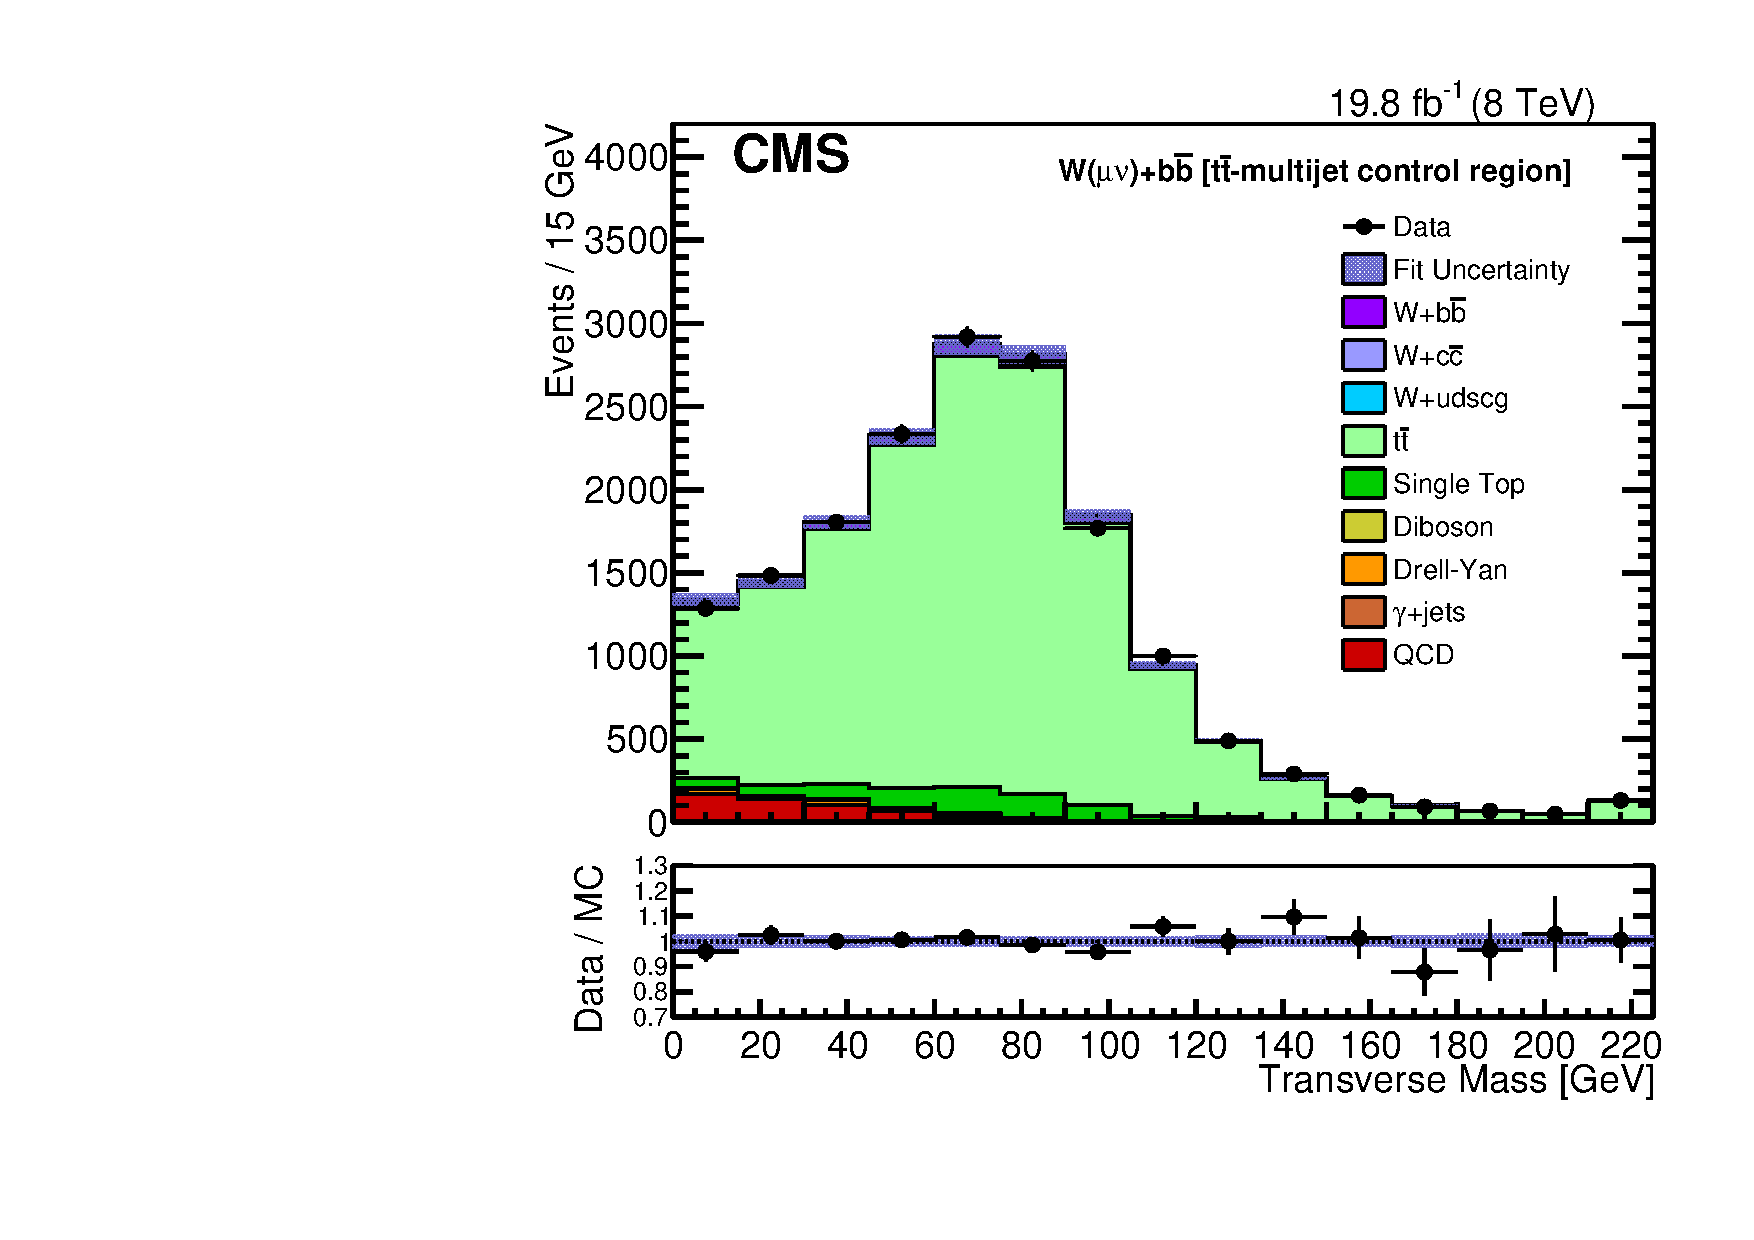
\includegraphics[width=0.45\textwidth]{pdfs/wbbxc/pape/poststep1_ttjjj_mt_mu} & 
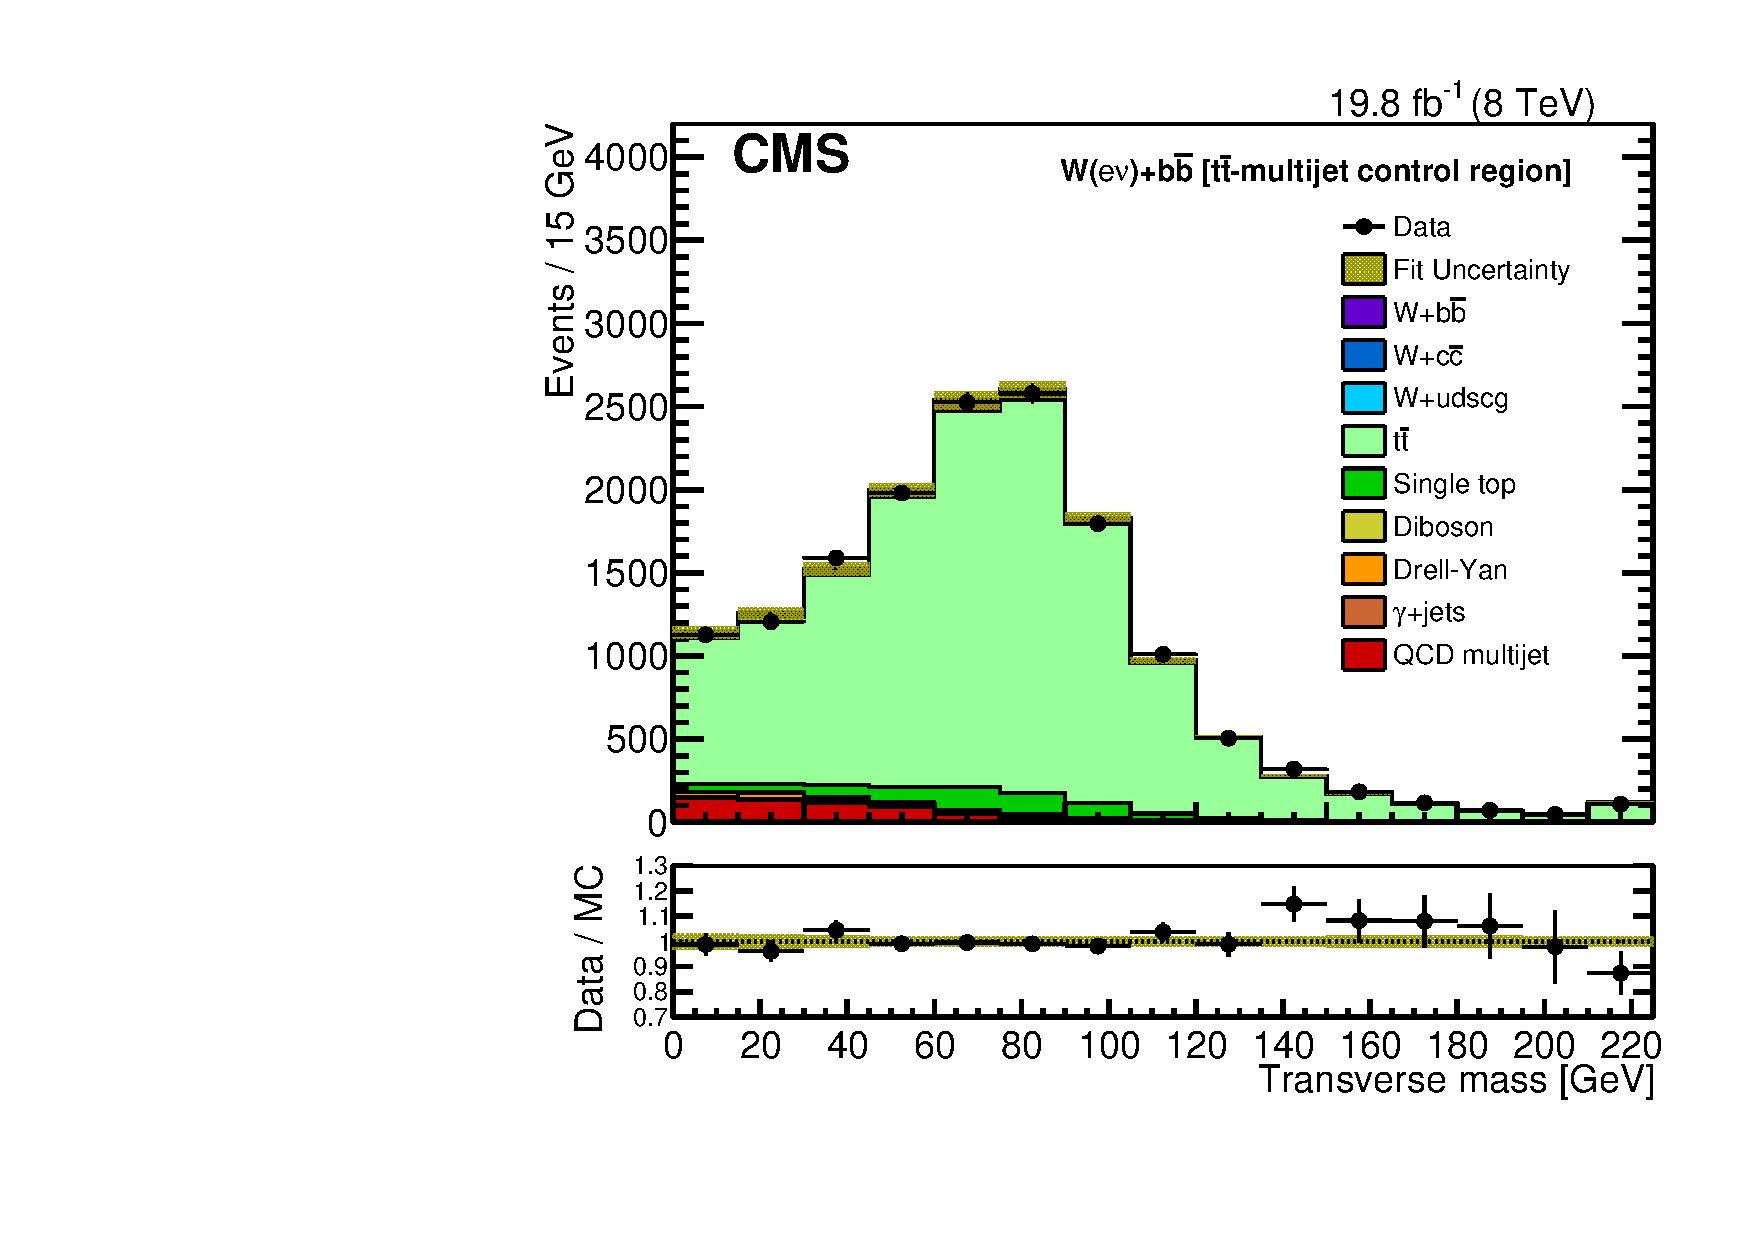
\includegraphics[width=0.45\textwidth]{pdfs/wbbxc/pape/poststep1_ttjjj_mt_ele} \\
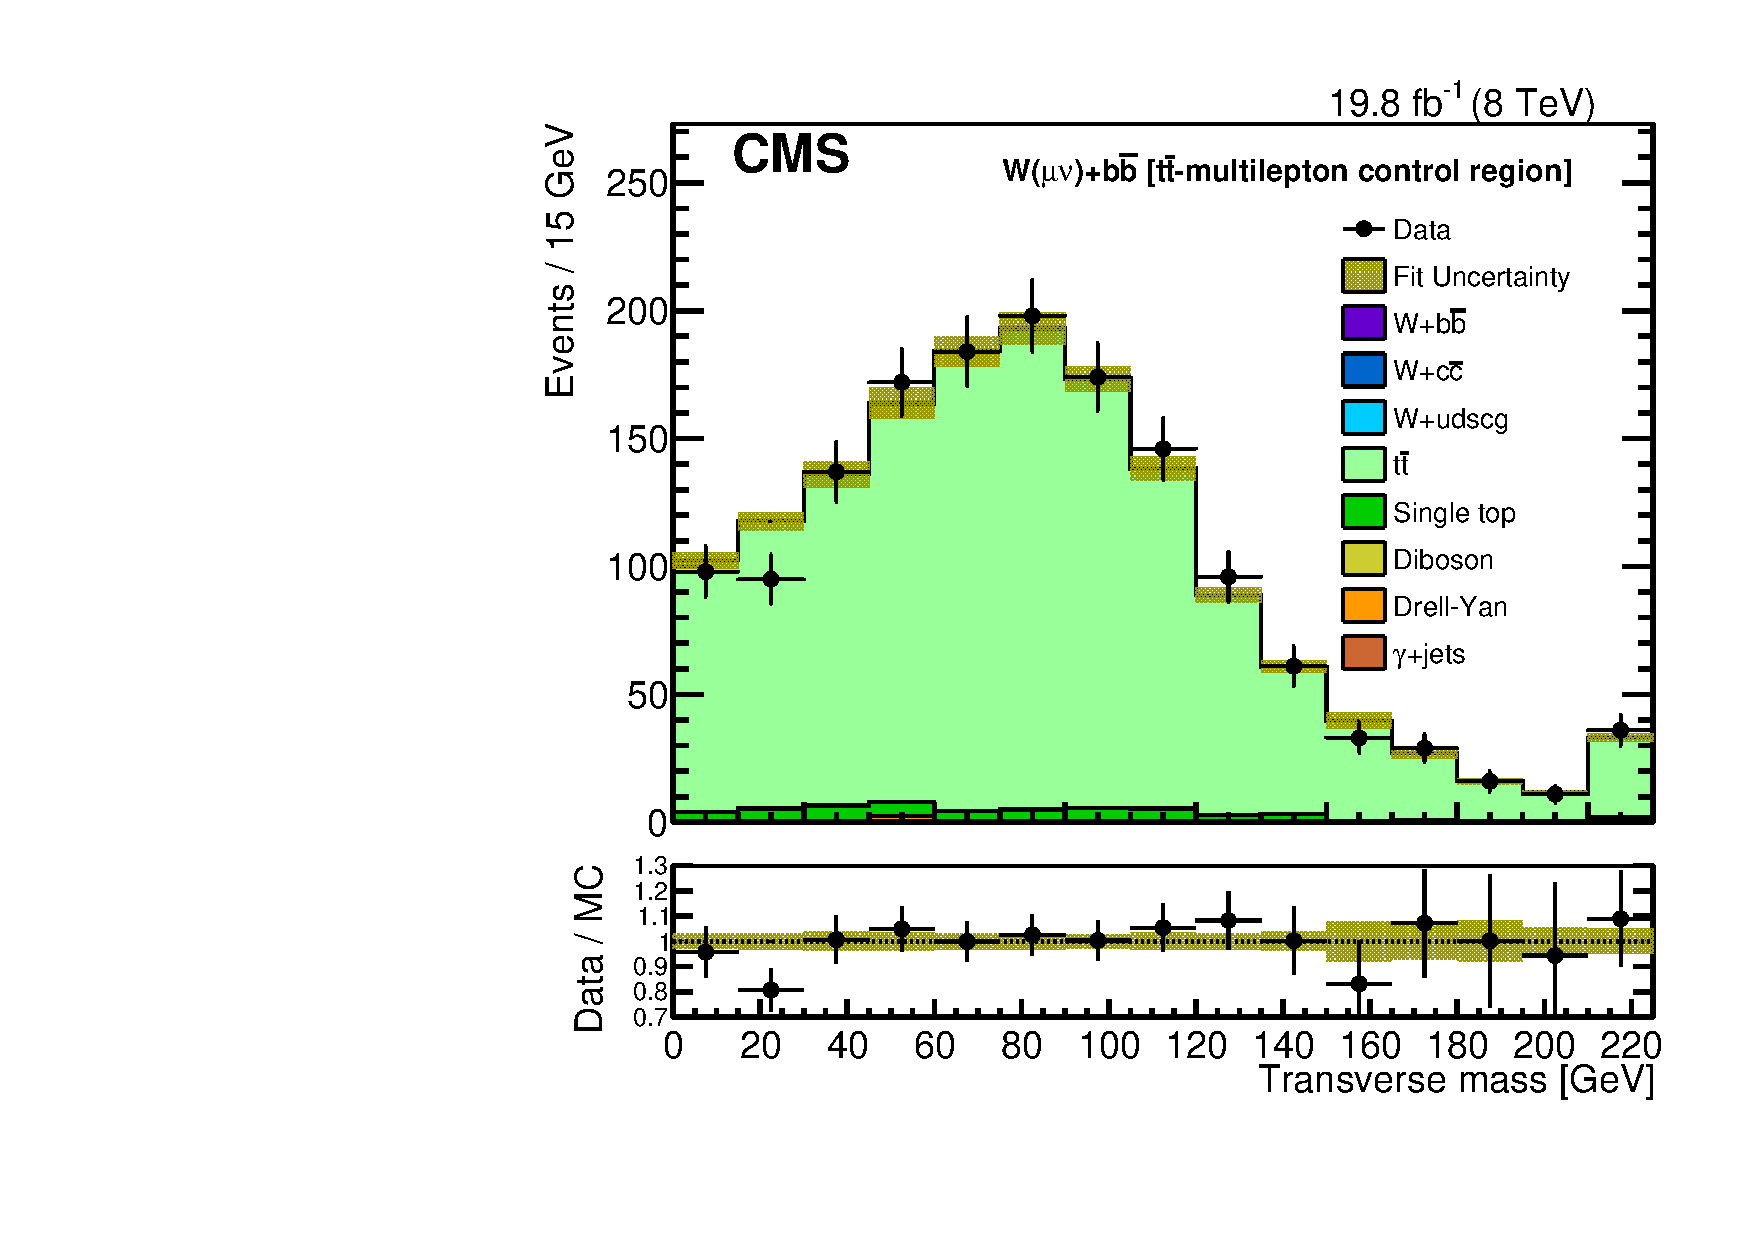
\includegraphics[width=0.45\textwidth]{pdfs/wbbxc/pape/poststep2_ttme_mt_mu} & 
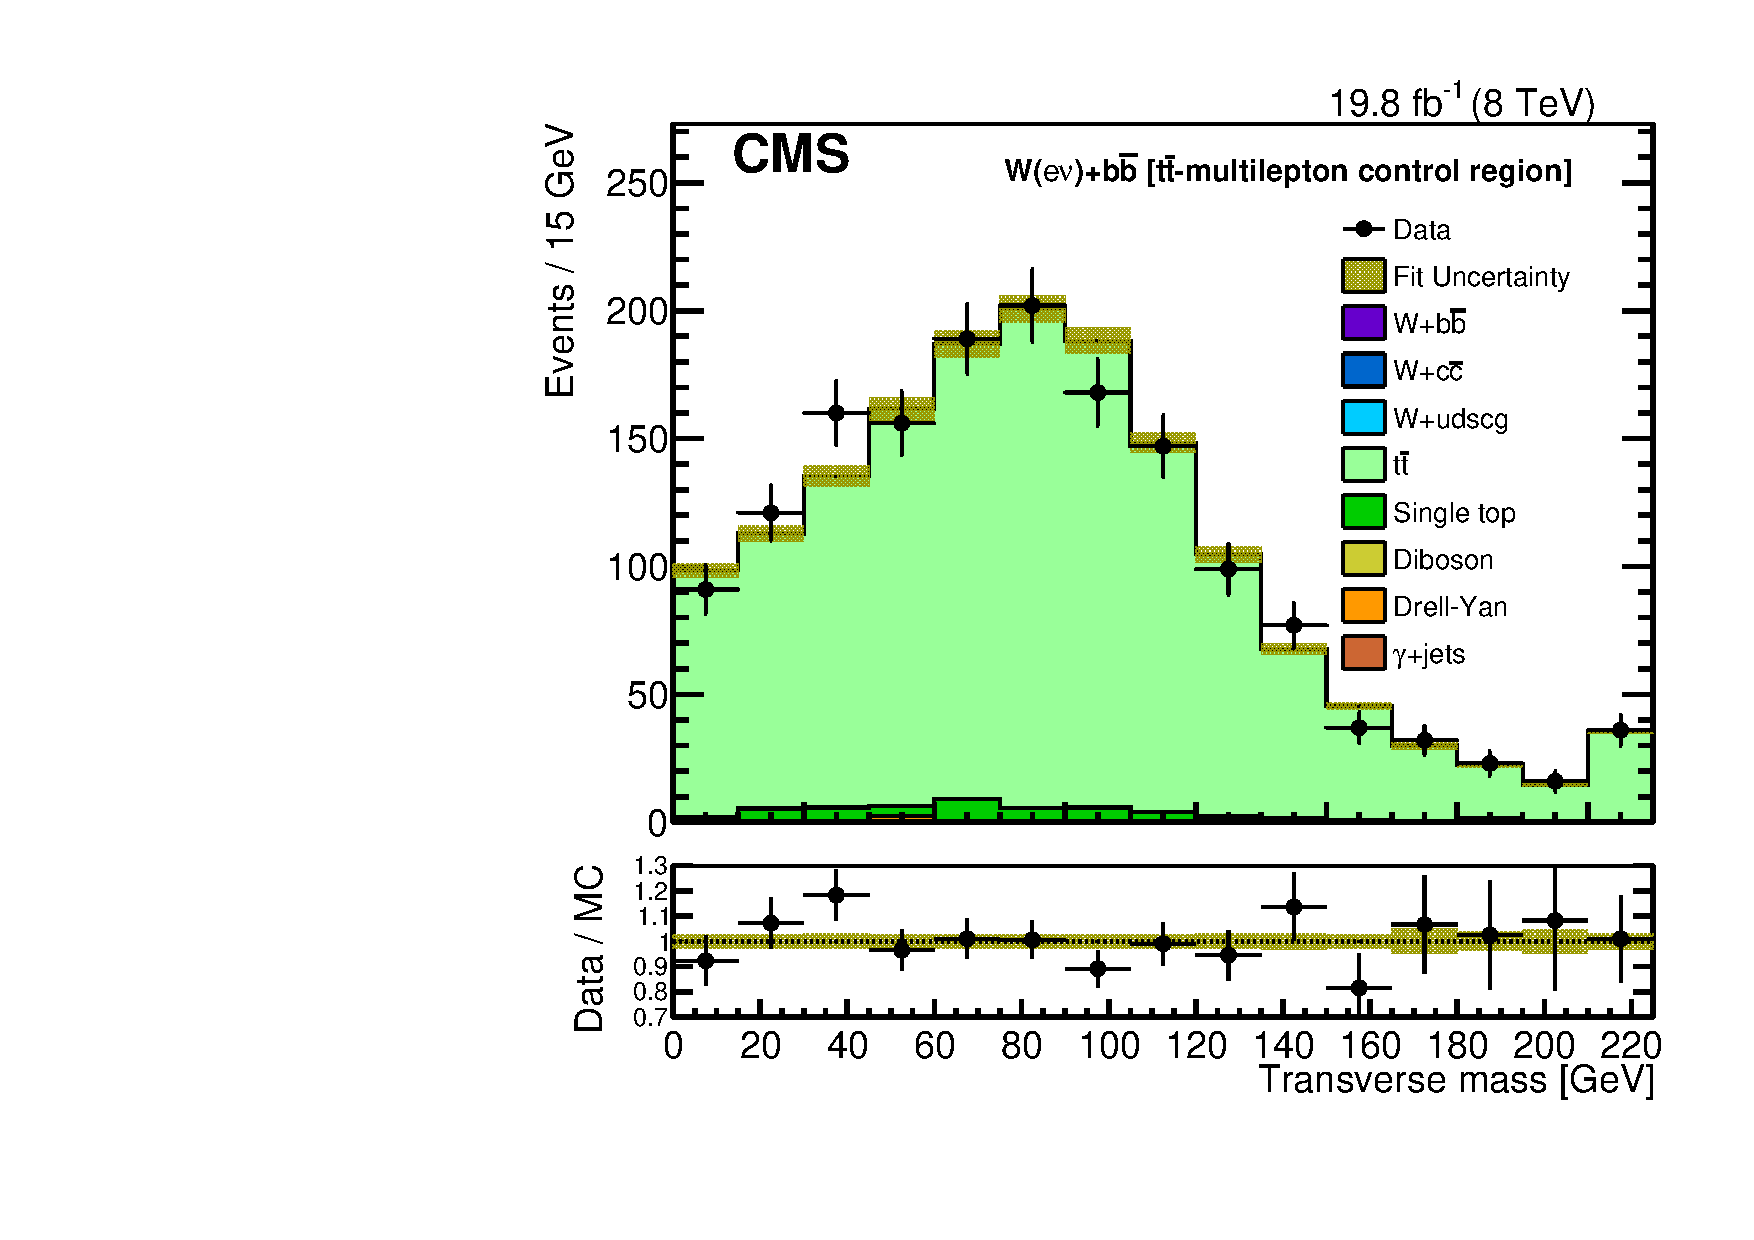
\includegraphics[width=0.45\textwidth]{pdfs/wbbxc/pape/poststep2_ttme_mt_ele} \\
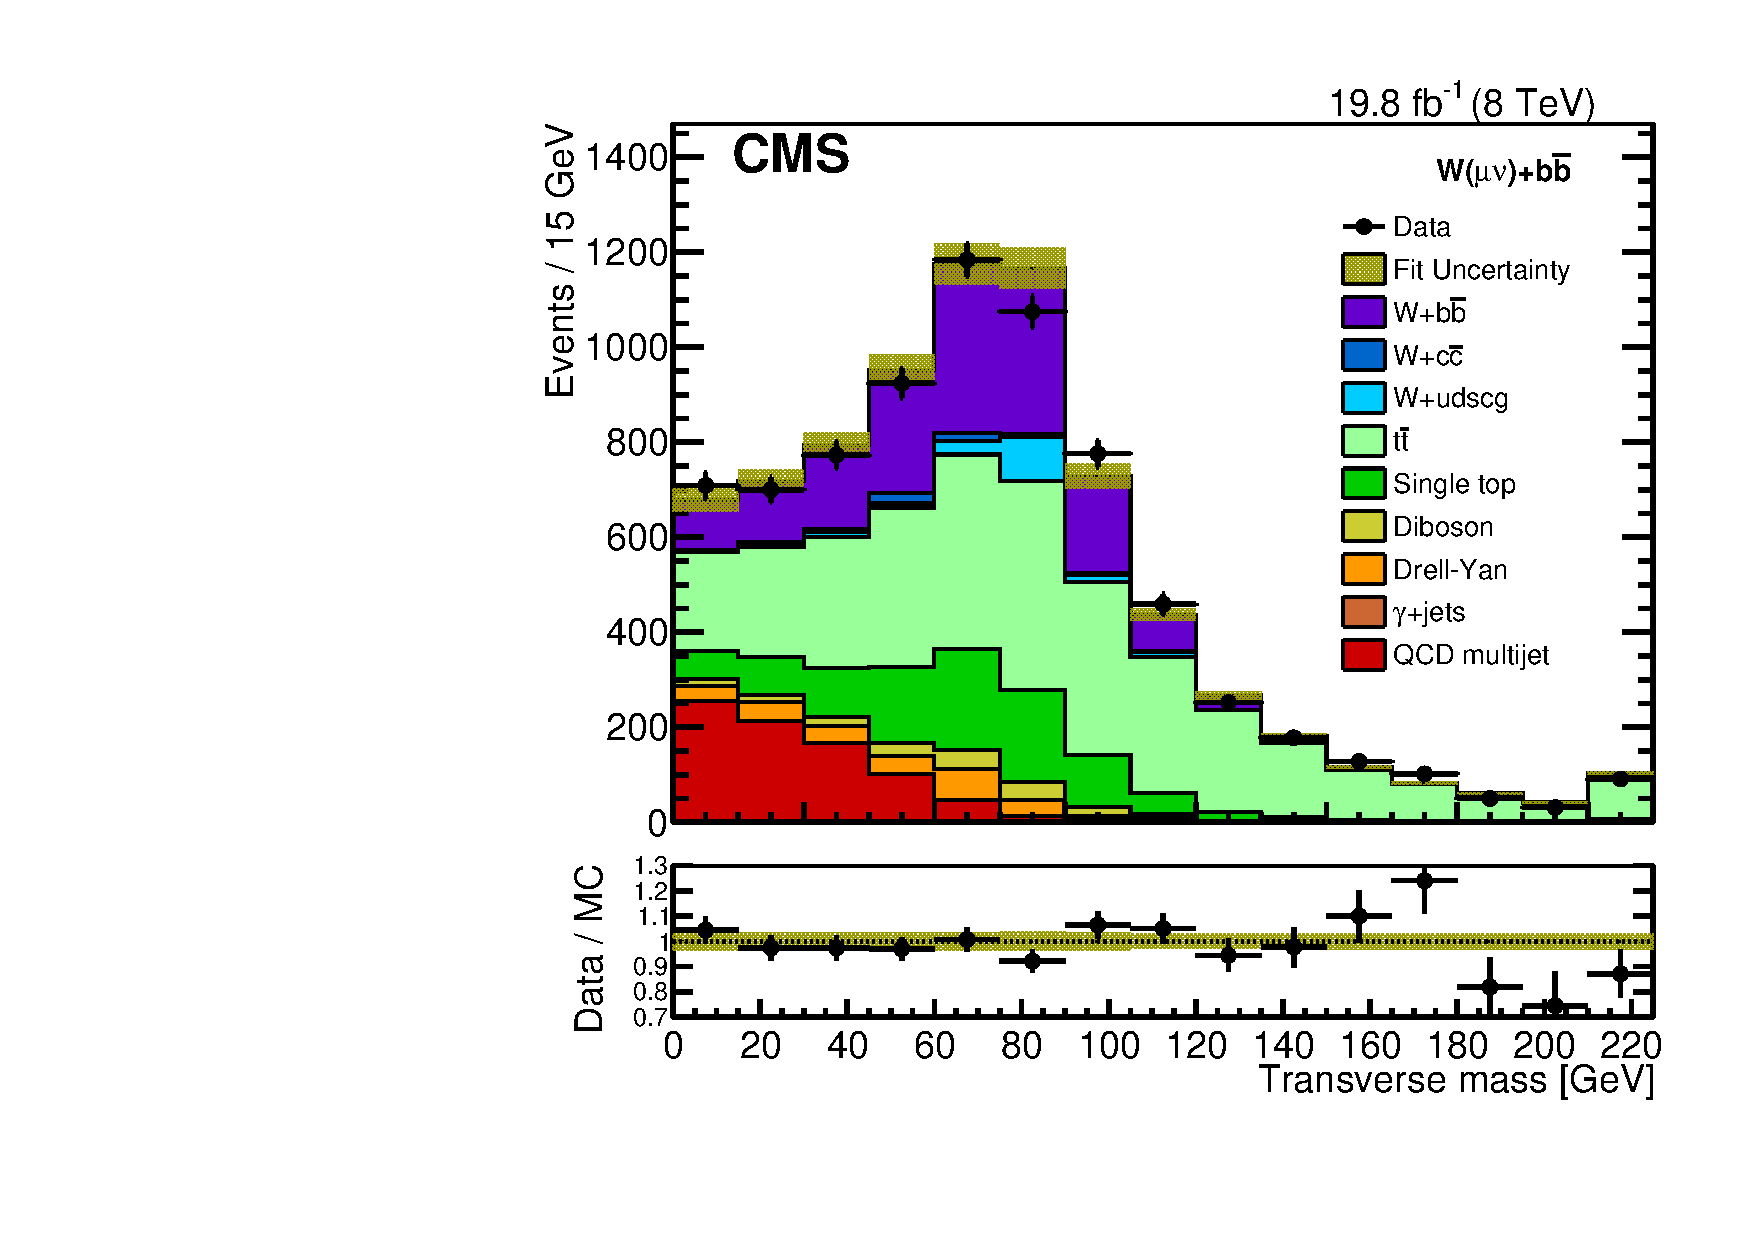
\includegraphics[width=0.45\textwidth]{pdfs/wbbxc/pape/postcfit_wbb_mt_mu} &
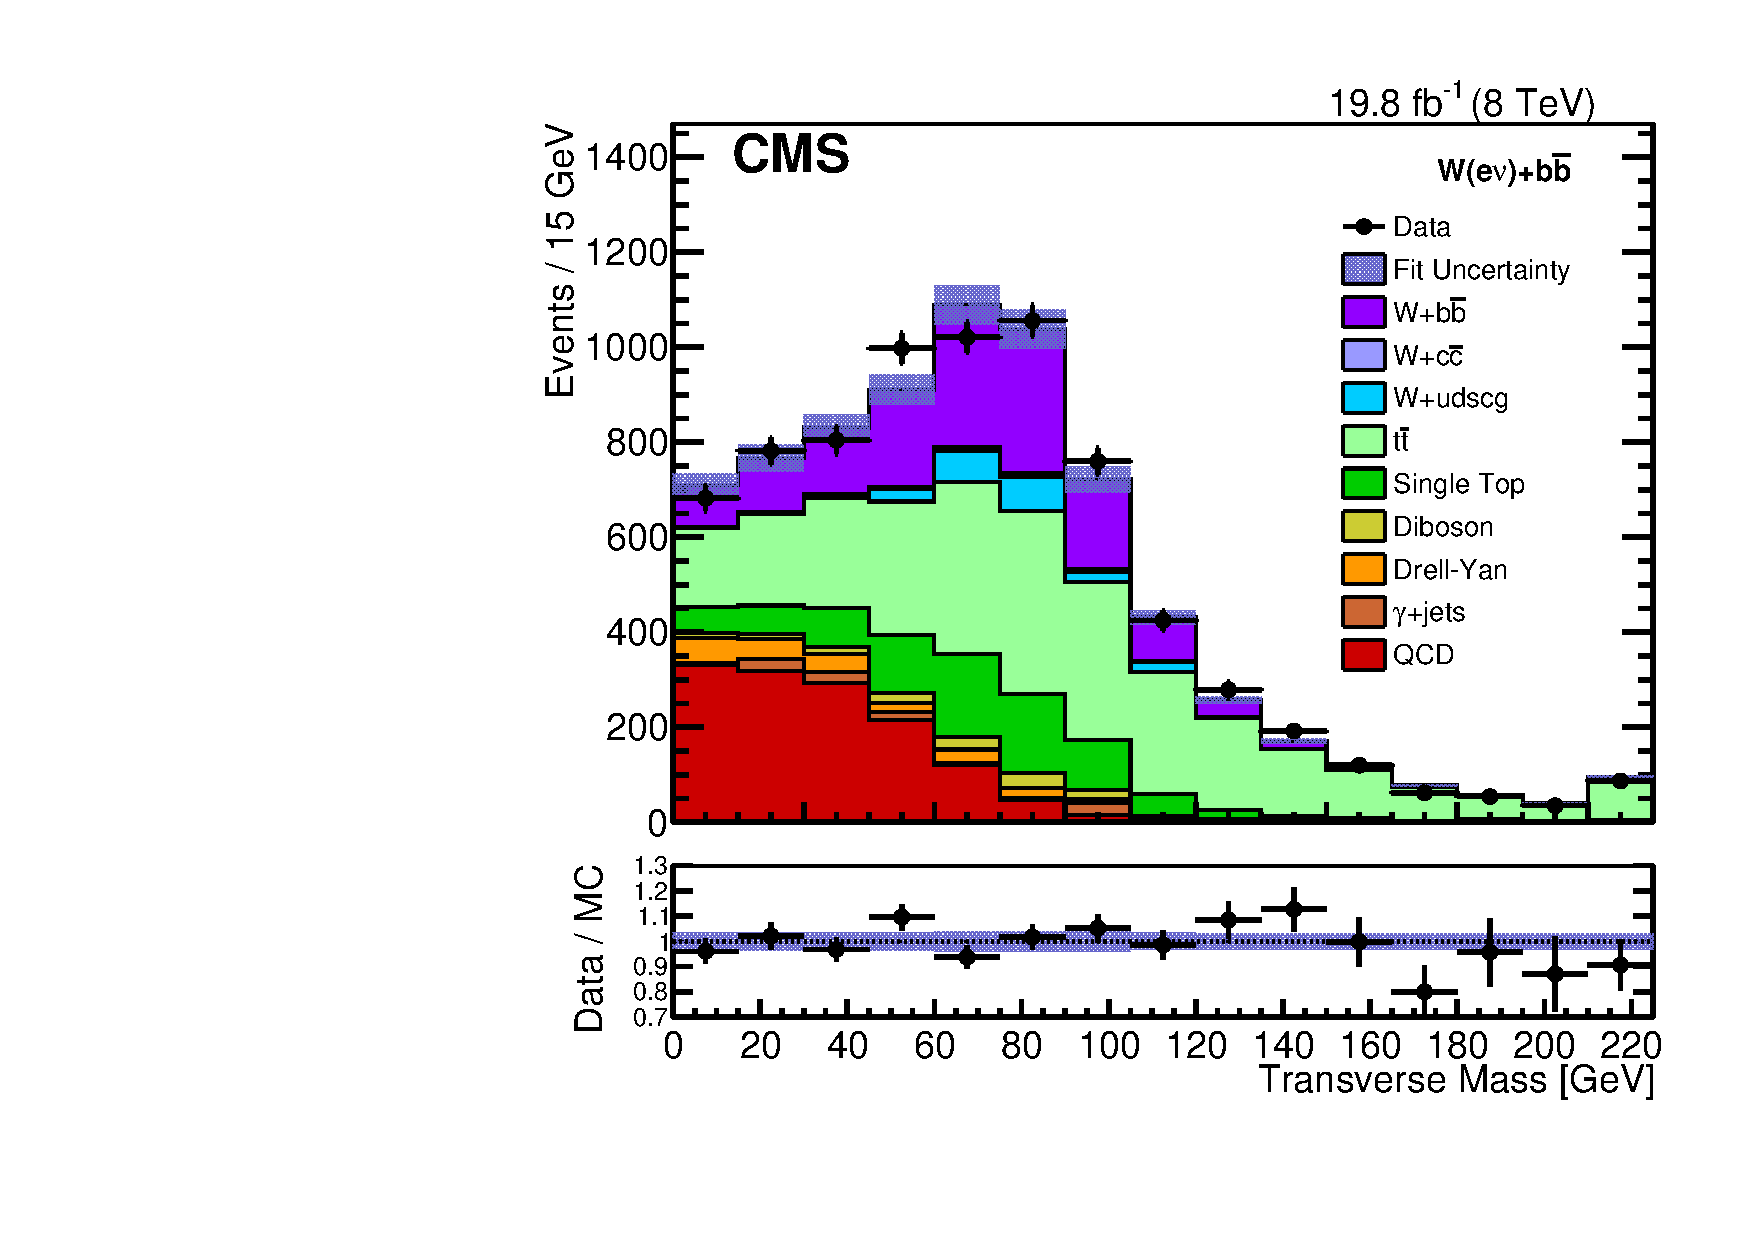
\includegraphics[width=0.45\textwidth]{pdfs/wbbxc/pape/postcfit_wbb_mt_ele}
\end{tabular}
\end{centering}
\label{fig:fittingplots}
\end{figure}


% dR(jj) and pT(l) postfit 
\begin{figure}[!htb]
\center
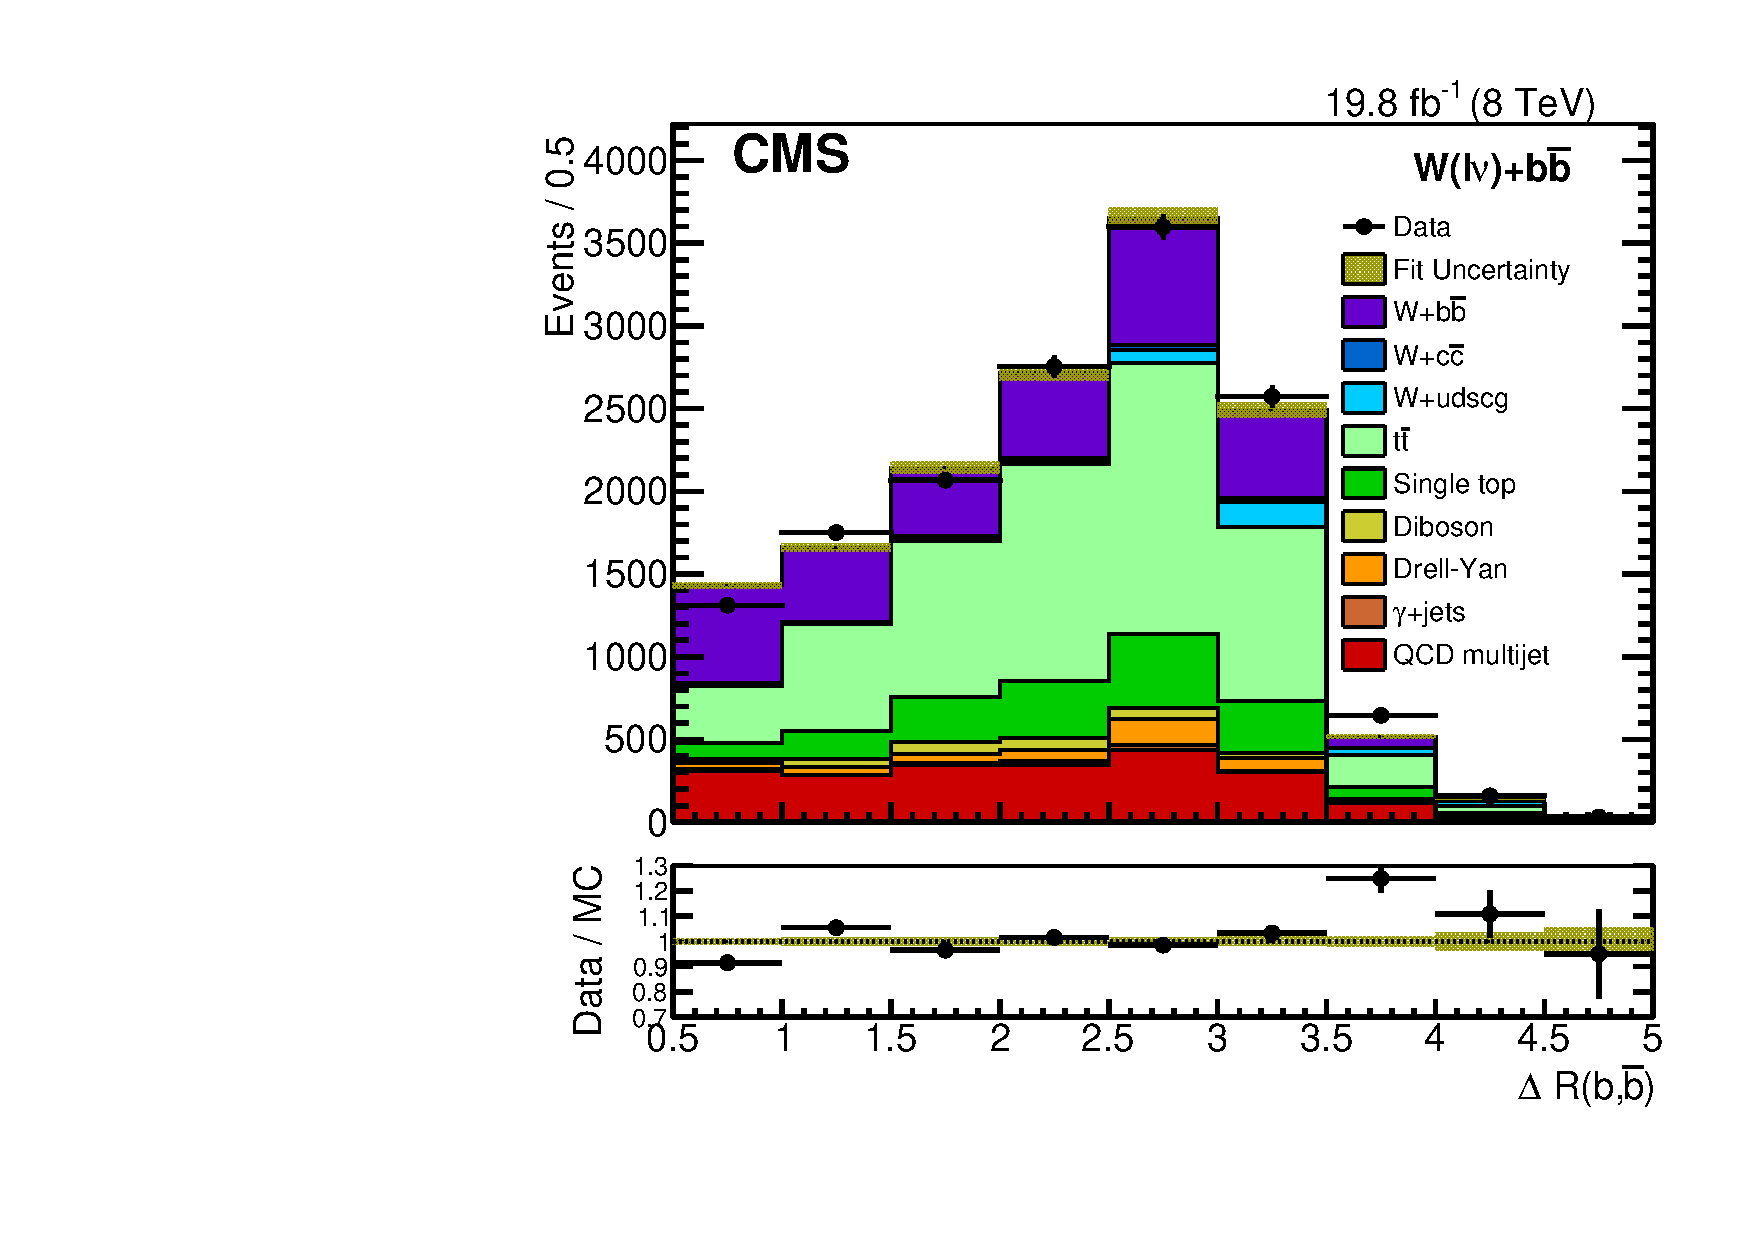
\includegraphics[width=0.49\textwidth]{pdfs/wbbxc/pape/postcfit_wbb_dRJ1J2}
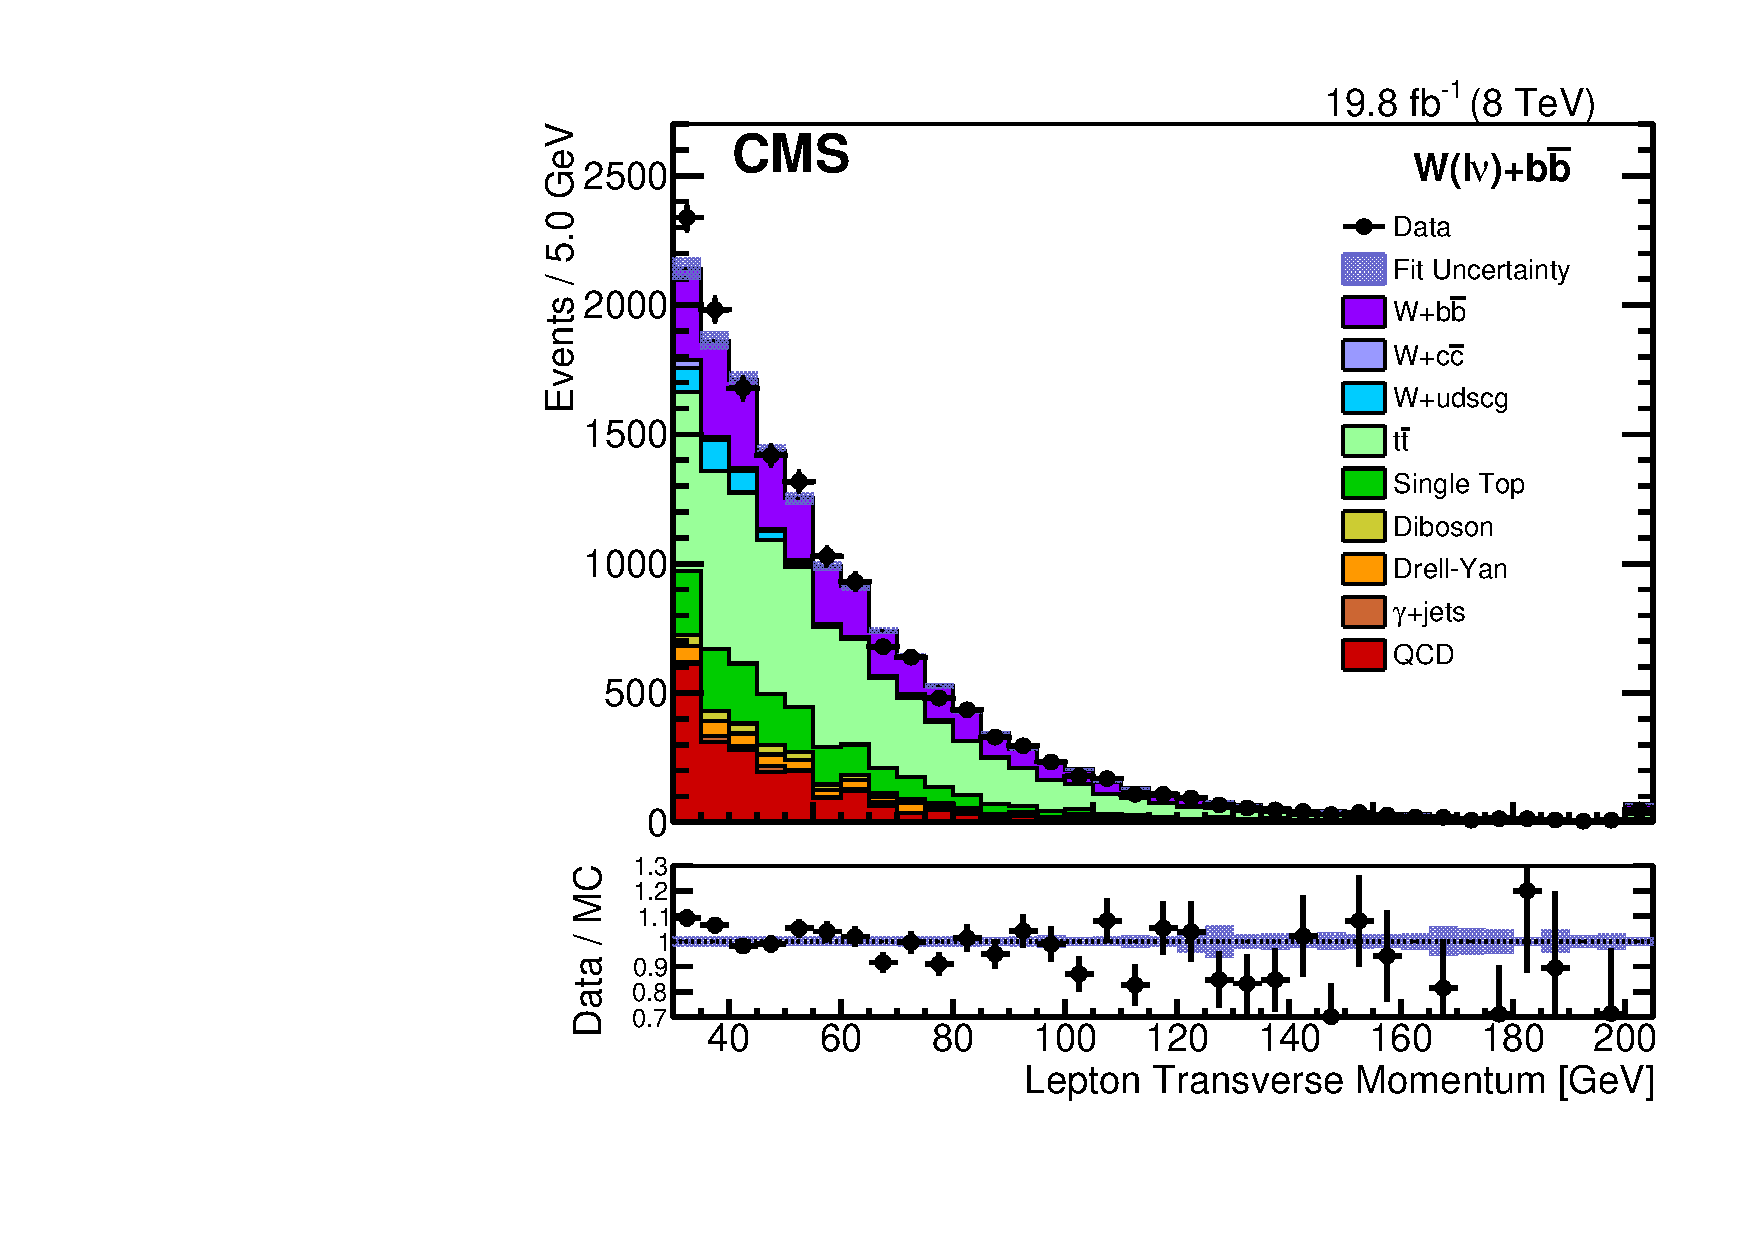
\includegraphics[width=0.49\textwidth]{pdfs/wbbxc/pape/postcfit_wbb_pTLep}
\caption[More variables in the \wbb signal region]{
  Distributions of $\Delta R(b\bar{b})$ and $\pt^\ell$ after
   applying the results from the fits to the simulation.
  The QCD background shape is taken from an $\mt<30$ GeV sideband and the
   muon and electron channels have been combined in these distributions.
  The last bin contains overflow events and
   the shaded area represents the total uncertainty in the simulation after the fit.
 }
\label{fig:postfit_drbb_ptl}
\end{figure}


\section{Cross Section and Comparisons}

The cross section for the process
 $\sigma(\ppwbblnbb)$,
 is derived from the signal strength measurement as obtained from the fit.
The cross section is written as

$$\sigma(\ppwbblnbb) = 
\frac{N^{\mathrm{Data}}_{\mathrm{signal}}}{A\cdot\epsilon\cdot \mathcal{L}} = 
\frac{N^{\mathrm{Data}}_{\mathrm{signal}}}{(N^{\mathrm{MC}}_{\mathrm{signal}}/N^{\mathrm{MC}}_{\mathrm{generated}})\cdot \mathcal{L}} =
%\frac{N_{\mathrm{signal}}}{N_{\mathrm{rec}}} \cdot \frac{N_{\mathrm{gen}}}{\mathcal{L}} = 
\alpha \sigma_{\mathrm{gen}}$$
 where
 $N^{\mathrm{Data}}_{\mathrm{signal}}$ is the number of observed signal events,
 $N^{\mathrm{MC}}_{\mathrm{signal}}$ is the number of expected signal events from simulation,
 $N^{\mathrm{MC}}_{\mathrm{generated}}$ is the number of generated events in the fiducial region,
 $A$, $\epsilon$ are the acceptance and efficiency correction factors,
 $\alpha$ is the measured signal strength in the given lepton channel, and
 $\sigma_{\mathrm{gen}}$ is the simulated fiducial cross section of the signal sample.

In this analysis, the fiducial cross section was calculated in the following manner:
 \MADGRAPH is used to compute the $\wbb$ cross section with fiducial cuts applied.
Then a k-factor for inclusive W production is applied, obtained from the ratio
of the inclusive W cross sections calculated with \FEWZ (at NNLO using the five-flavour
\CTEQ6M PDF set) and with Madgraph.
%In this analysis, the cross section used was calculated with \textsc{fewz} at NNLO
% using the five-flavor \CTEQ6M PDF set on the inclusive $\wjets$ sample.
The product $A\cdot\epsilon$ is 13~(11)\% in the
 muon (electron) channels and results from the
 combined effect of the efficiency from
 lepton identification requirements (80\%), and $b$ tag efficiency (40\% per jet).
The uncertainty on this product is 10\% as listed in the bottom row of
 Table \ref{tab:input_unc_wbb}, which was calculated by varying the PDF
 set using the LHAPDF/PDF4LHC \cite{LHAPDF,Botje:2011sn,Alekhin:2011sk,Ball:2012cx}
 prescription considering
 PDF sets from \CTEQ, \MSTW, \NNPDF, and \HERA
 as well as varying the
 choice of scales
 $\mu_{\mathrm{F}}$, $\mu_{\mathrm{R}}$ simultaneously
 up and down by a factor of two.
Varying the PDFs and the choice of scale is a way to 
 to estimate the dependence of the measured cross section on the 
 choices of these parameters.
 

The $\wbb$ cross section is measured within a fiducial volume, which is defined by
requiring leptons with $\pt > 30\GeV$ and $\abs{\eta}<2.1$ and exactly two $b$-tagged jets of
 $\pt > 25\GeV$ and $\abs{\eta}<2.4$.
The measured cross sections are presented in Table \ref{tab:crosssections}.
The combination of the muon and electron measurements is done using a simultaneous fit to both channels,
 taking into account correlations between different sources of uncertainties.

\begin{table}[!h]
\begin{center}
\caption{
 Measured cross sections in the muon, electron, and combined lepton channels.}
\label{tab:crosssections}
 \begin{tabular}{l|c}
 Channel        & $\sigma(\ppwbblnbb)$ pb \\
\hline
 Combined & $  0.64 \pm 0.03 \mathrm{(stat)} \pm 0.10 \mathrm{(syst)} \pm 0.06 \mathrm{(theo)} \pm 0.02 \mathrm{(lumi)} $ \\
\hline 
     Muon & $  0.62 \pm 0.04 \mathrm{(stat)} \pm 0.11 \mathrm{(syst)} \pm 0.06 \mathrm{(theo)} \pm 0.02 \mathrm{(lumi)} $ \\
 Electron & $  0.70 \pm 0.05 \mathrm{(stat)} \pm 0.15 \mathrm{(syst)} \pm 0.07 \mathrm{(theo)} \pm 0.02 \mathrm{(lumi)} $ \\
 \end{tabular}
\end{center}
\end{table}



% 
The measured cross sections are compared to theoretical predictions from
 \MCFM \cite{Campbell:2010ff, Badger:2010mg}
 with the {\MSTW2008} PDF set, as well as from
 %with the {\MSTW2008} NNLO PDF set, as well as from
 \MADGRAPH5
 interfaced with \PYTHIAs in the four- and five-flavour schemes and
 \MADGRAPH5 with \PYTHIAe \cite{ref:Pythia8} in the four-flavour scheme.
In the five-flavour scheme, the PDF set {\CTEQ6L} was
 used and \PYTHIAs was run using {TuneZ2*}.
The two four-flavour samples were produced using
 a NNLO PDF set interfaced with %NNLO23\_lo\_as\_0130\_qed
 \PYTHIA (version 6 in one sample, version 8 in the other)
 in the {CUETP8M1} tune.

% motivation
Comparisons between the results of calculations performed
 under different assumptions provide important feedback
 on the functioning and validity of the techniques employed.
Differences in predictions arising from the modelling of
 $b$ quarks as massive or massless are possible, as are
 variations in predictions arising from the use of different
 showering packages (\PYTHIAs vs.\ \PYTHIAe) or matrix element
 generators (\MADGRAPH vs.\ \MCFM).
In the phase space explored here, these predictions are all
 very close in their central value and agree with each other
 well within their respective uncertainties.

% $b$ -> B
The \MCFM cross section calculation is
 performed at the level of parton jets and thus
 requires a hadronization correction.
The multiplicative hadronization correction factor $0.81\pm0.07$
 is calculated using the \MADGRAPH + \PYTHIAs sample
 and agrees well with a
 similar factor calculated in the $7\TeV$ Z+b analysis
 calculated as $0.84\pm0.03$  \cite{Chatrchyan:2014dha}.
This factor is determined by 
 taking the ratio of the predicted cross sections
 in a given sample after having undergone a simulation
 of the hadronization process, and using
 jets identified at the particle list level.
The correction factor is obtained for
 jets computed excluding neutrinos from the particle list, aparticles
 such jets are closer in kinematics
 to particle jets at the detector level.
The uncertainty reflects both the statistics of the
 \MADGRAPH + \PYTHIAs sample as well as a comparison with the
 \MADGRAPH + \PYTHIAe sample.

% DPS
The \MCFM and four-flavour \MADGRAPH predictions do not account for
 \wbb production where the \bbbar system comes from multiple parton scattering.
CMS simulations of \MADGRAPH + \PYTHIA events that include
 double parton interactions (DPIs) reproduce the $\wjets$ data \cite{Chatrchyan:2013xxa},
 therefore a \MADGRAPH + \PYTHIAe sample of a $\w$ boson produced in association with a
 \bbbar pair coming from DPS
 was generated to study the effect on the fiducial cross section.
Using this dedicated sample, an additive correction $\sigma_{\mathrm{DPS}}$
 is estimated to be $0.06\pm0.06$ pb, where the uncertainty
 is conservatively assigned to be 100$\%$ of the value.

% PDF/scale uncertainty
The uncertainty in the theoretical cross sections arising
 from the choice of PDF is also accounted for,
 using the LHAPDF/PDF4LHC \cite{LHAPDF,Botje:2011sn,Alekhin:2011sk,Ball:2012cx}
 prescription in which
 PDF sets from \CTEQ, \MSTW, \NNPDF, and \HERA are considered.
Uncertainties in the theoretical cross section due to the
 choice of scale are also estimated by varying the scales
 $\mu_{\mathrm{F}}$, $\mu_{\mathrm{R}}$ simultaneously
 up and down by a factor of two.

The resulting cross section predictions in the fiducial
 phase space at the hadron level and including the estimated
 hadronization and DPS corrections when needed
 are compared in Fig. \ref{fig:xc_comparison}
 with the measured value.
Within one standard deviation the predictions agree with the measured cross section.
The results also agree within one standard deviation with previously published $\wbb$
 measurements at 7 \TeV, where
 data are found to be well described by the same predictions.

\begin{figure}[htbp]
\caption[Cross section comparison for \wbb and generators]{
 Comparison between the measured \ppwbblnbb cross section and 
  various QCD predictions.
 The orange band indicates the uncertainty 
  in the given sample associated with PDF choice
  and the yellow band represents the uncertainty
  associated with DPI.
 The labels 4F and 5F refer to the four- and five-flavour
  PDF schemes, and 
  in the case of the \MADGRAPH + \textsc{\PYTHIA6} (5F) sample,
  the effects of DPI are already included in the generated
  samples so the DPI correction is not needed.
 The measured cross section is also shown with associated uncertainties.
 }
\center
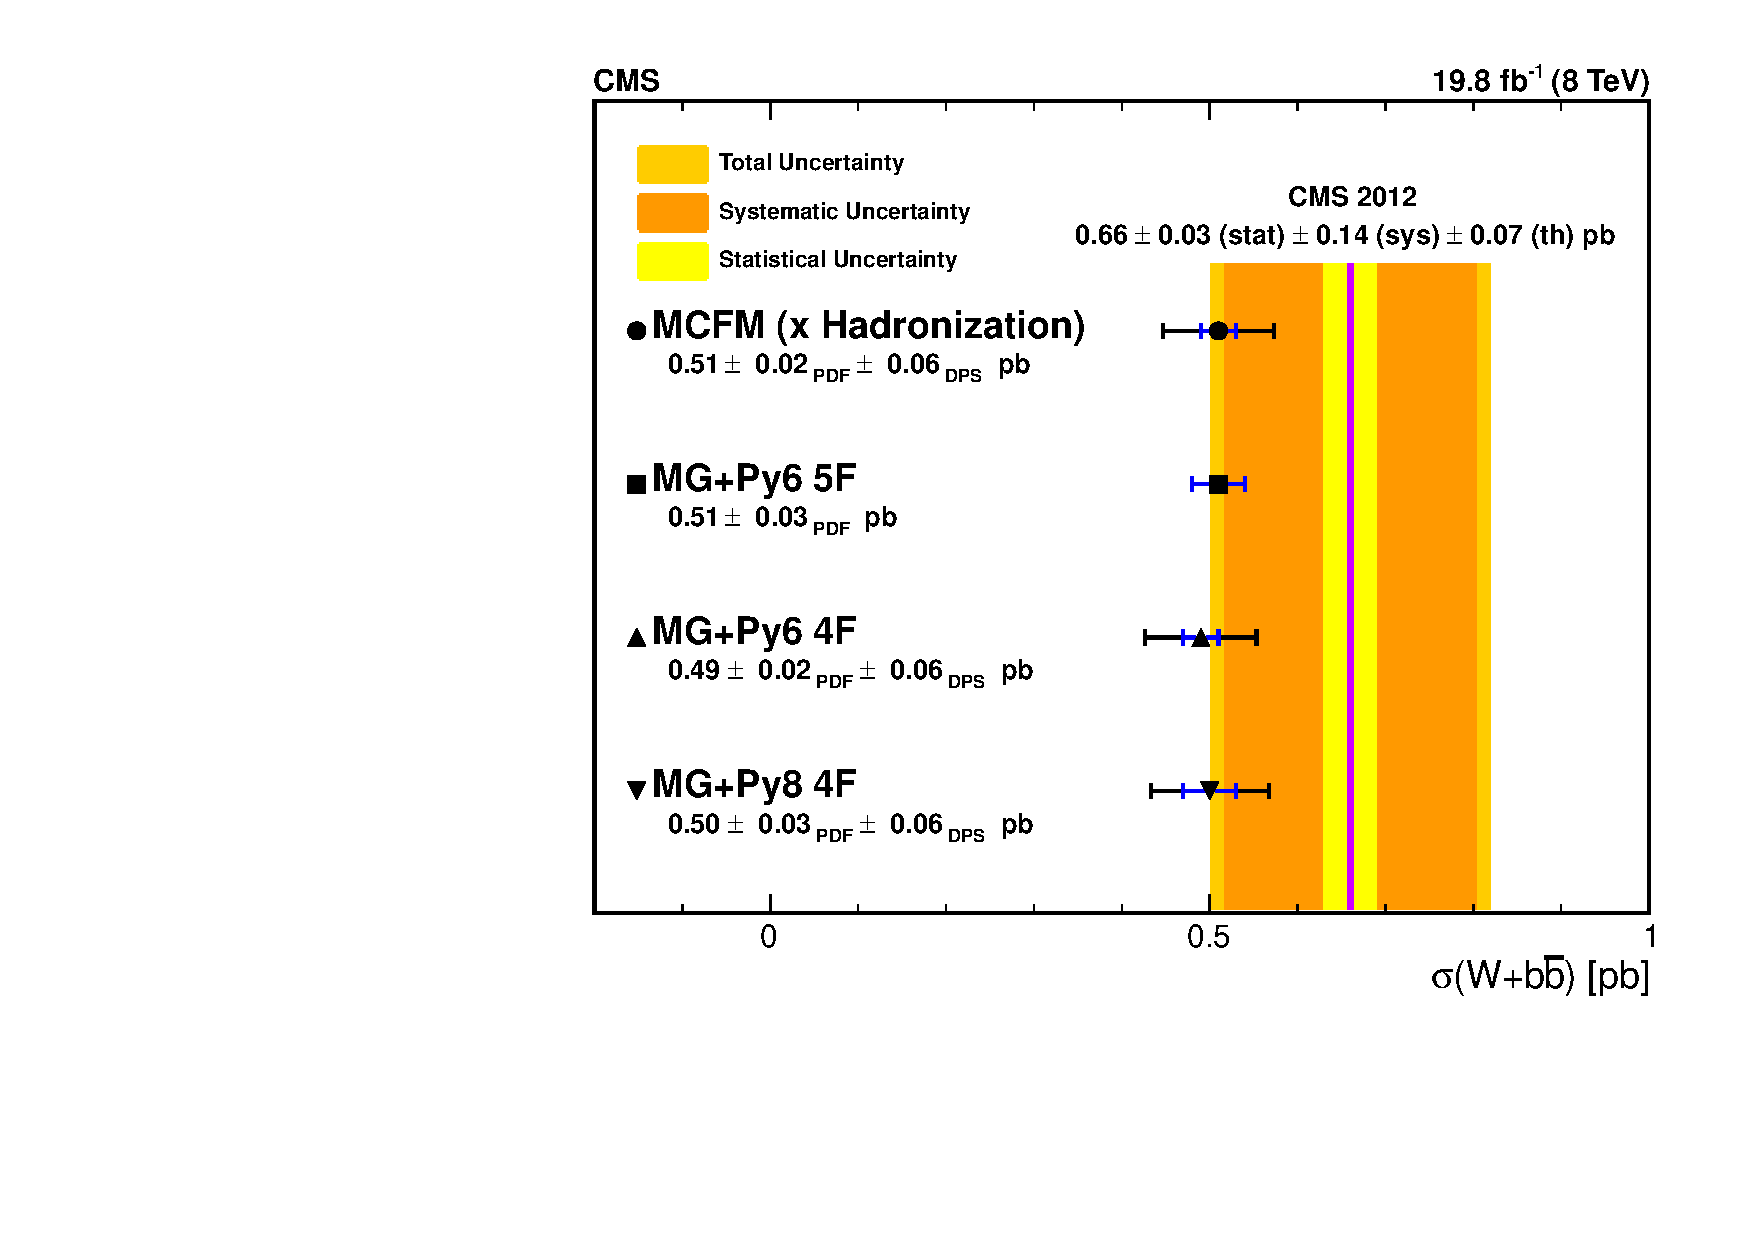
\includegraphics[width=0.7\textwidth]{/Users/rhombus/CMS/Thesis/thesis/pdfs/wbbxc/pape/MCXC_Comparison}
\label{fig:xc_comparison}
\end{figure}

